%%%%%%%%%%%%%%%%%%%%%%%%%%%%%%%%
%
%  CLICIDE
%
%%%%%%%%%%%%%%%%%%%%%%%%%%%%%%%%
\chapter{Corpus pour l'évaluer des méthodes de recherches d'information multimédia}

\section{Corpus d'images pour la recherche d'instance dans un musée d'art}
\label{chap:corpus}

Le premier corpus que nous avons construit se nomme "CLICIDE". 
Il est composé de photographies de peintures issues de l'exposition permanente du musée de Grenoble\footnote{http://www.museedegrenoble.fr/}. 
Ce musée propose au visiteur principalement des peintures occidentales entre le XIV$^{\text{\`e}me}$ et le XXI$^{\text{\`e}me}$ siècle. 
Il y a donc une grande variabilité de styles et d'époques (expressionnisme, impressionnisme, art sacré, pop art, ...). 
La figure~\ref{fig:exempleClicide} présente quelques images montrant la diversité des œuvres de cette collection.

\begin{figure}[htb]
   \begin{minipage}[c]{.3\linewidth}
      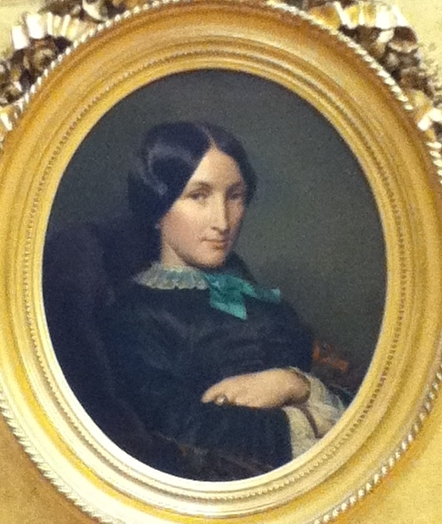
\includegraphics[width=\linewidth]{figures/15R-3.JPG}
   \end{minipage} \hfill
   \begin{minipage}[c]{.3\linewidth}
      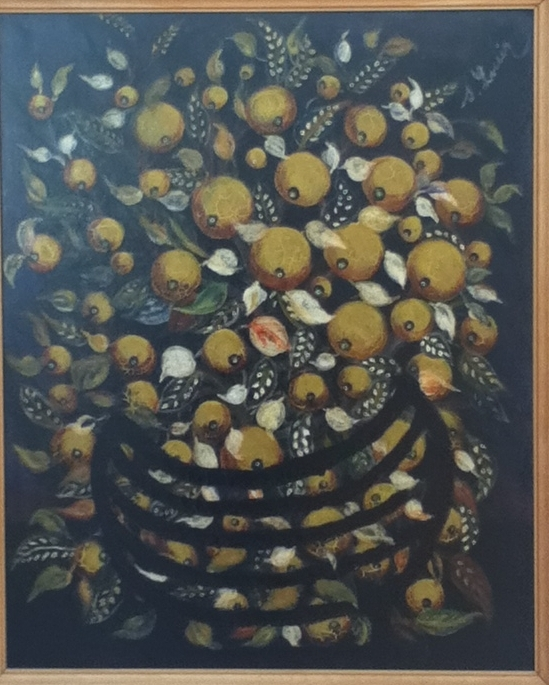
\includegraphics[width=\linewidth]{figures/34C-7.JPG}
   \end{minipage} \hfill
   \begin{minipage}[c]{.3\linewidth}
      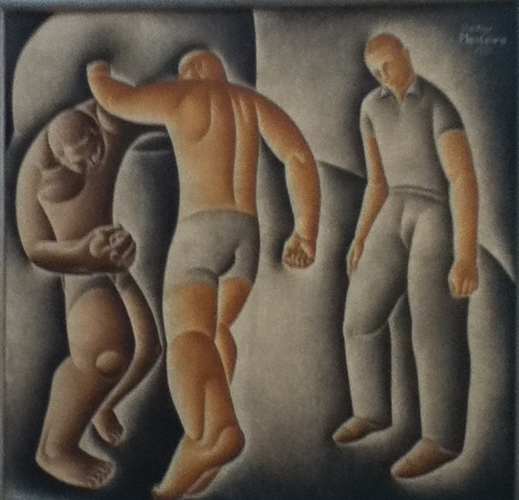
\includegraphics[width=\linewidth]{figures/35G-4.JPG}
   \end{minipage} \hfill
    \caption{Images tirées de la collection Clicide. de gauche à droite : ``Portrait de la mère du docteur Bordier'' de Hippolyte Flandrin, ``Les fruits'' de Séraphine de Senlis, ``O Combate'' de Vicente do Rego Monteiro. }
    \label{fig:exempleClicide}
\end{figure}

Le corpus Clicide est composé de 3425 photographies, qui représentent 473 œuvres du musée. 
Les œuvres ont été photographiées par 3 personnes, en utilisant un appareil reflex et des téléphones portables. Chaque œuvre est photographiée plusieurs fois (une image de l'œuvre complète, et des images correspondant à des parties de l'œuvre). 
Pour chaque œuvre considérée, une photographie du cartouche est également stockée. 
Chaque image d'œuvre est associée à un identifiant unique sous la forme suivante: $<$numéro de salle$>$$\_$$<$numéro de l'œuvre dans la salle$>$\_$<$numéro d'indice$>$. Ces images sont rognées manuellement afin de limiter la proportion d'arrière-plan.

De plus, 177 photographies, de 143 œuvres, tirées aléatoirement de la collection initiale, sont utilisées comme requêtes (et donc retirées du corpus). 
Ces images sont prises de différents points de vus et avec différentes proportions d'arrière-plan.
La figure~\ref{fig:exempleRequeteClicide} présente une image requête (à gauche) et une image du même objet tirée du corpus (à droite).

\begin{figure}[htb]
\centering
\begin{subfigure}{0.4\linewidth}
	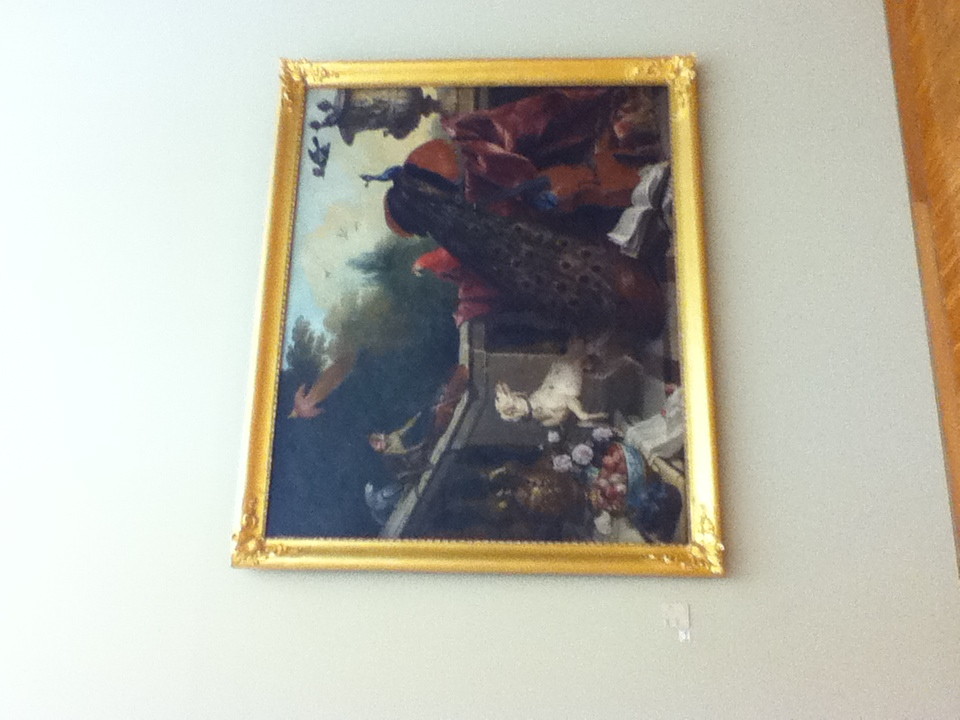
\includegraphics[height=0.95\textwidth,angle=-90]{figures/12G-0428.JPG}
	\caption{Exemple de requête}
\end{subfigure}


\begin{subfigure}{0.4\linewidth}
	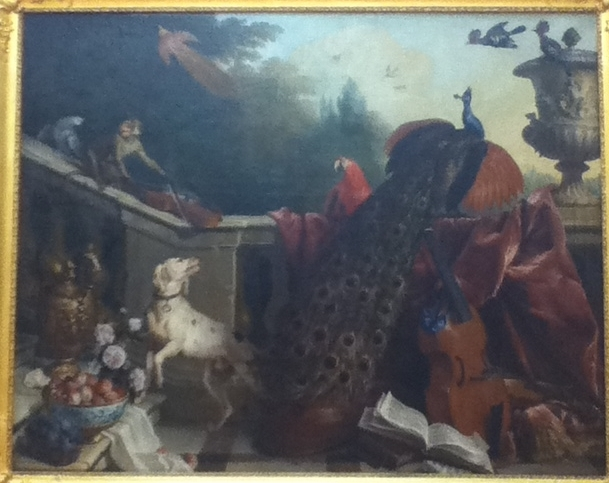
\includegraphics[height=0.95\textwidth]{figures/12G-12.JPG}
	\caption{Image référence du corpus}
\end{subfigure}

    \caption{Photographies d'``Animaux Fleurs et Fruits'' d'Alexandre-François Desportes tirée de Clicide.}
 \label{fig:exempleRequeteClicide}
\end{figure}



%%%%%%%%%%%%%%%%%%%%%%%%%%%%%%%%
%
%  GaRoFou
%
%%%%%%%%%%%%%%%%%%%%%%%%%%%%%%%%
\section{Corpus de recherche d'image et de vidéo dans un musée d'héritage culturel}
\label{sec:garofou}

Une deuxième collection a été réalisée avec le musée Gallo-Romain de Fourvière\footnote{http://www.museegalloromain.grandlyon.com/} qui est un musée français, localisé à Lyon, portant sur la civilisation Gallo-Romaine. 
Situé près d'un théâtre romain sur la colline de Fourvière, ce musée présente dans sa collection permanente, des objets pré-romains, romains, celtes (inscriptions, statues, joaillerie, objets de la vie courante), comme le montre les exemples de la figure~\ref{fig:exempleFourviere}.

\begin{figure}[htb]
\centering
    \begin{minipage}[c]{.2\linewidth}
      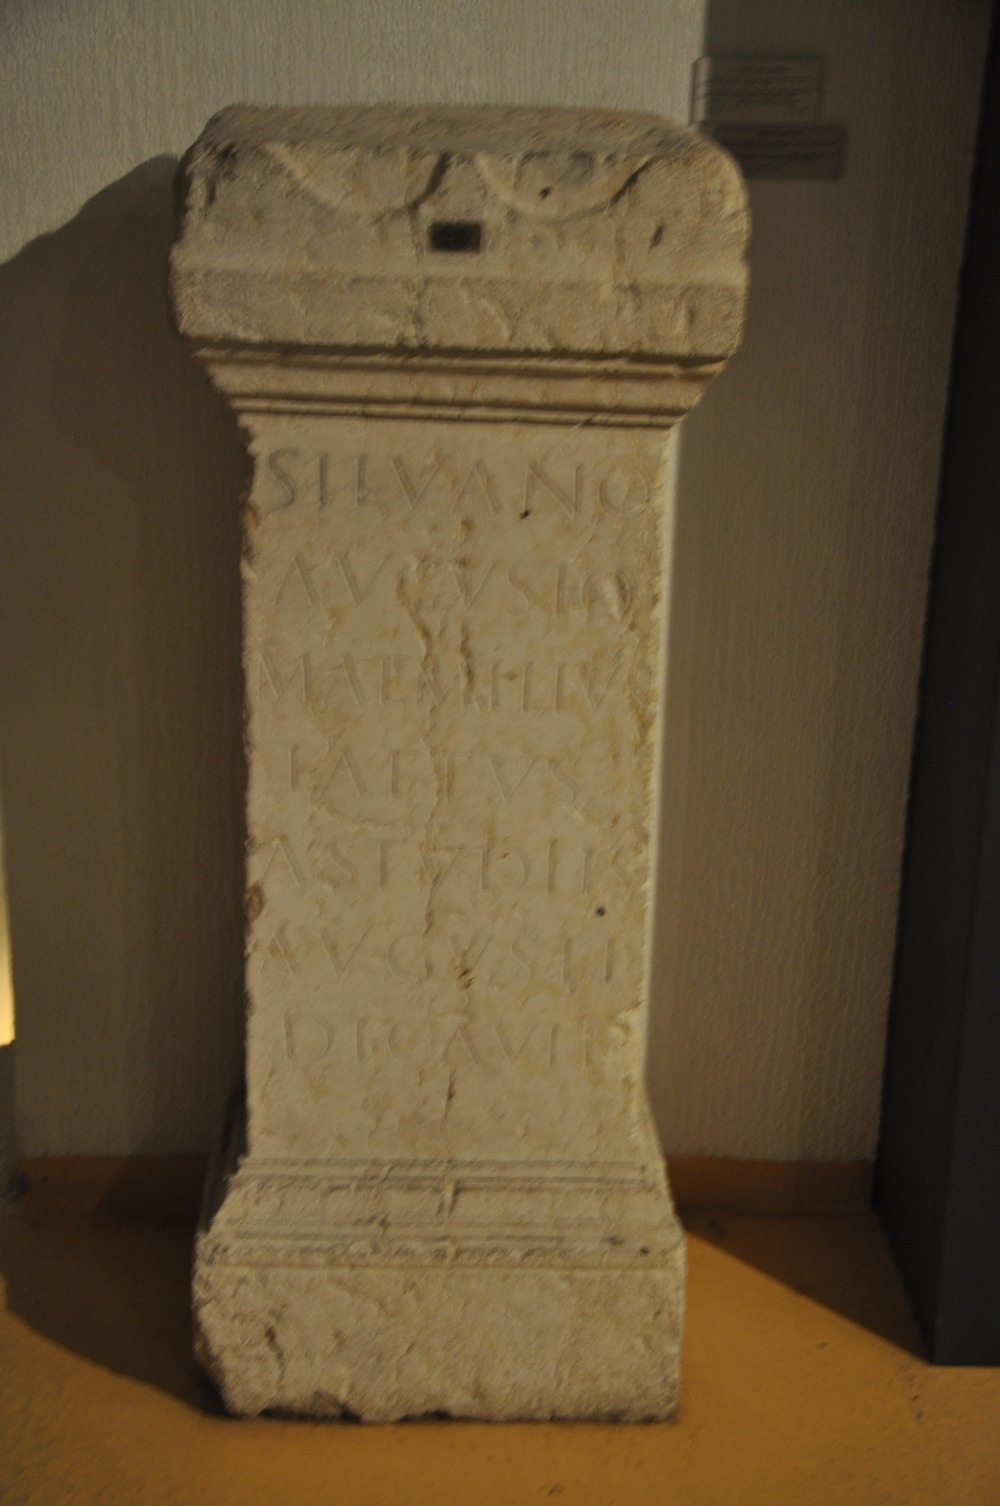
\includegraphics[width=\linewidth]{figures/B-016-01.jpg}
   \end{minipage}
   \begin{minipage}[c]{.2\linewidth}
      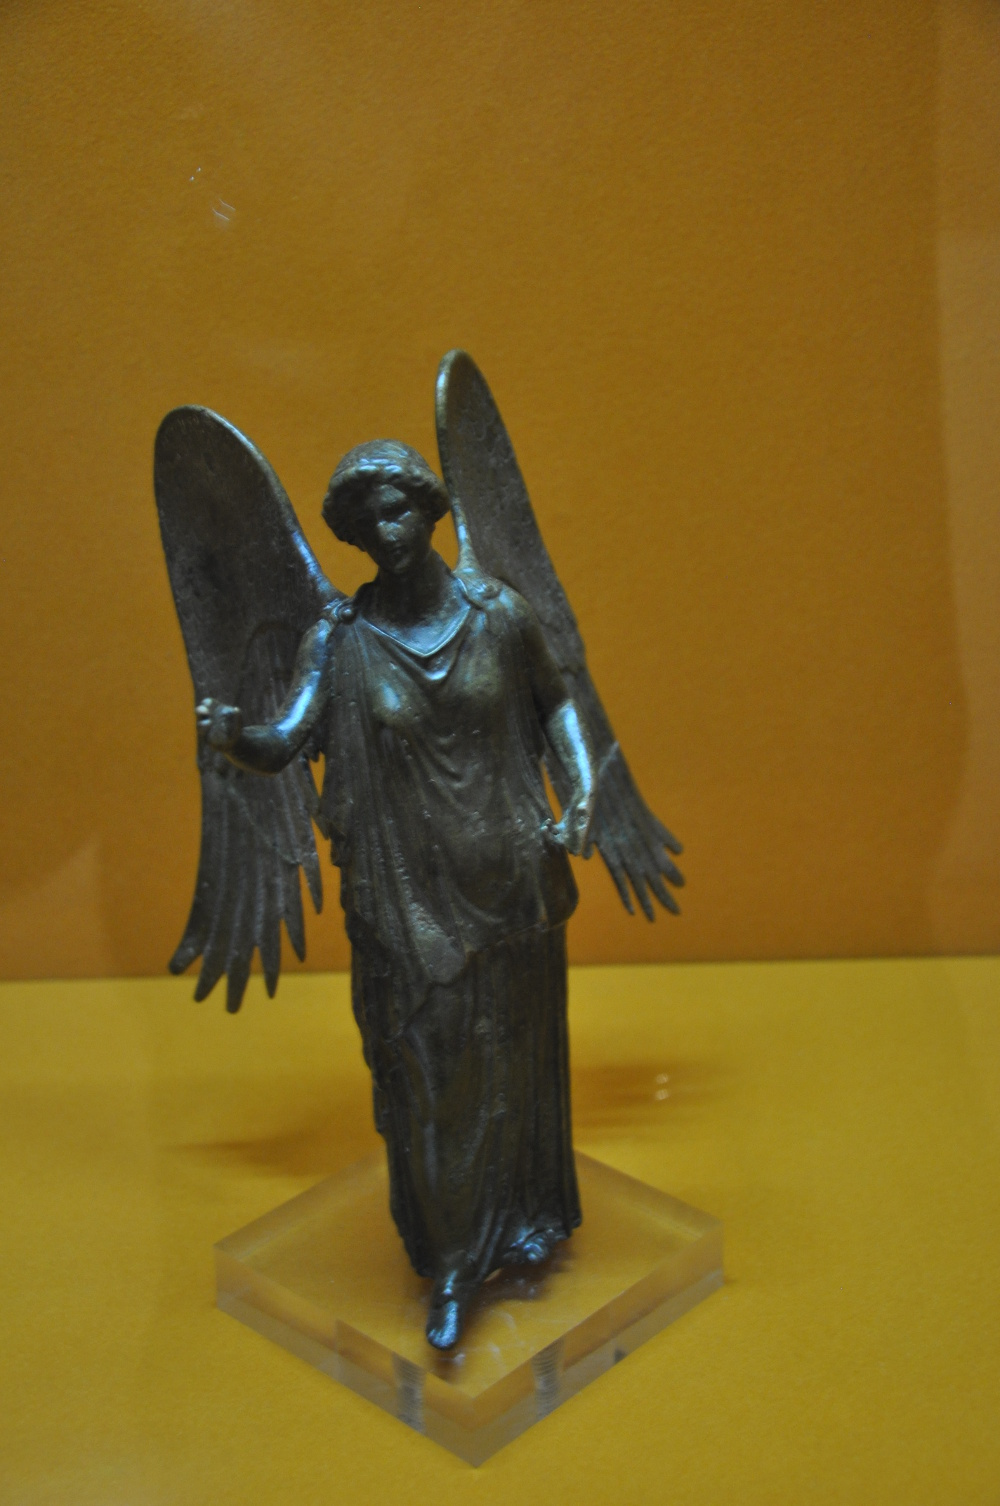
\includegraphics[width=\linewidth]{figures/A_019_00.jpg}
   \end{minipage}
   \begin{minipage}[c]{.2\linewidth}
      \includegraphics[height=\linewidth,angle=-90]{figures/DSC_0174.JPG}
   \end{minipage}
    \caption{Photographies de la collection de Fourvière. De gauche à droite: une stèle, une statue et une poterie.}
  	\label{fig:exempleFourviere}
\end{figure}

La collection appelée {\bf GaRoFou}, pour musée {\bf Ga}llo {\bf Ro}main de {\bf Fou}rvière, est composée d'images fixes (GaRoFou\_I) et de vidéos (GaRoFou\_V).

\section{Garofou\_I}
\label{sec:garoufoui}

GaRoFou\_I contient au total 1252 photographies, prises par des appareils reflex, de 311 œuvres. Parmi ces images, 1068 sont des images du corpus, et 184 des images requêtes sélectionnées aléatoirement. Sur les 311 œuvres, 166 sont représentées dans l'ensemble des requêtes. Les photographies requêtes ont différents points de vue, qui ne sont pas forcément présents dans le corpus. Chaque image du corpus est identifiée par l'œuvre qui y est visible, auquel est associé le {\it type} de l'œuvre parmi: stèle (roches gravées, colonnes, ...), statue (sculptures, reliefs, ...), poterie, et autres (pièces, joaillerie, ...). Les œuvres sont identifiées par un triplet numéro de niveau (de A à D), le numéro d'œuvre dans le niveau, et un numéro d'image de l'œuvre suivant le format suivant:$<$numéro de niveau$>$$\_$$<$numéro de l'œuvre$>$$\_$$<$numéro d'image de l'œuvre$>$. Les images d'une même œuvre sont donc identifiées spécifiquement. 

\section{Garofou\_V}
\label{sec:garoufouv}

La partie vidéo de la collection Garofou est composée de 11 vidéos qui correspondent à des visites de différents étages du musée. Ces visites ont été effectuées par 5 personnes différentes, le même jour, avec une caméra fixée au dessus de la tête. Le détail sur ces vidéos est présenté dans le tableau~\ref{tab:video_garofou}. Dans ce tableau, nous détaillons en particulier les étages (notés de $A$ à $D$) du musée, la durée totale des vidéos brutes dans lesquelles les personnes ne sont pas forcément devant une œuvre, les durées durant lesquelles l'annotation manuelle a déterminé que des œuvres étaient le centre d'intérêt des visiteurs, le nombre d'œuvres correspondantes qui peut contenir des redondances car une personne peut se focaliser plusieurs fois sur une œuvre, ainsi que le nombre d'œuvres uniques vues.
Associés à chaque vidéo, les objets visibles qui ont attiré l'attention du visiteur sont indiqués par leur horodatage d'apparition et de disparition (en {hh:mm:ss} par rapport au début de vidéo). Pour générer ces annotations, nous avons développé une interface spécifique sur la base de la structure d'annotation du projet CAMOMILE~\cite{poignant2016camomile}, dont un exemple est présenté en figure~\ref{fig:annotation}.

\begin{table}[htb]
    \centering
    \begin{tabular}{| c | c | c | c | c | c |}
    \hline 
    étage & \# vidéos & durée  & durée avec & \# d'œuvres & \# œuvres  \\
      	  &           & totale & œuvre      & regardées   & uniques 	   \\
    \hline    
    \hline    
    A & 4 & 66'55''  & 38'35'' & 157 & 59\\
    B & 2 & 31'21''  & * 14'44'' & 77 & 56\\
    C & 3 & 30'51''  & * 17'35'' & 63 & 37\\
    D & 5 & 57'34''  & * 25'06'' & 115 & 63\\
    \hline    
    \hline    
  	total & 11 & 186'41'' & 96'00'' & 412 & 215 \\
    \hline
    \end{tabular}
    \caption{Vidéos de la collection GaRoFou\_V.}
    \label{tab:video_garofou}
\end{table}

\begin{figure}
\centering
    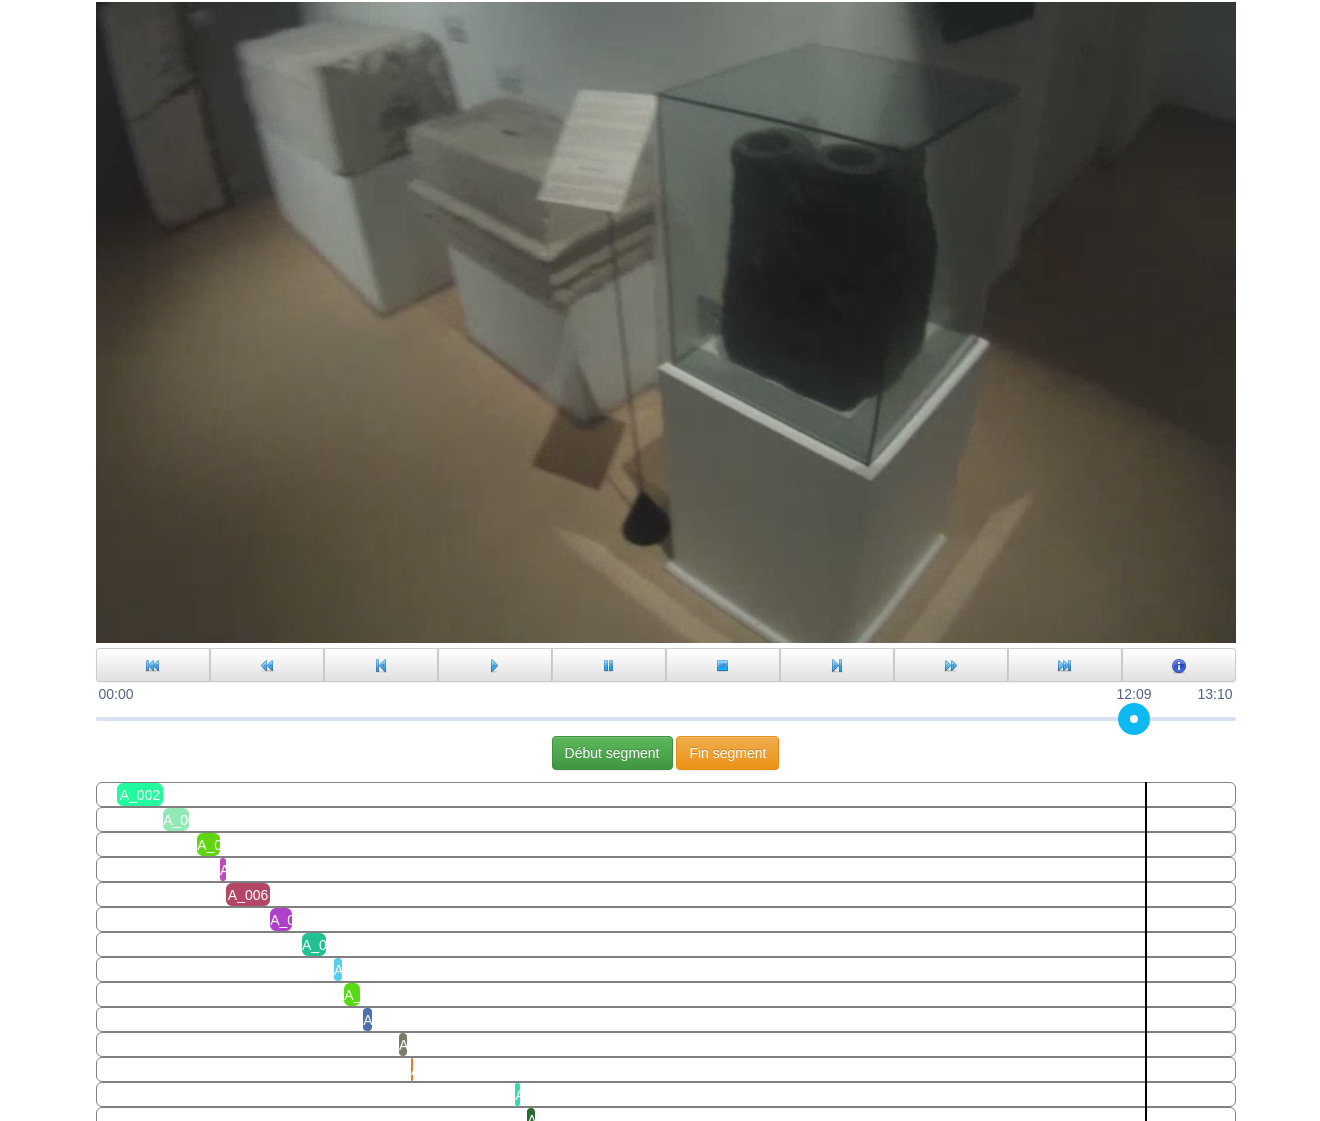
\includegraphics[width=0.9\linewidth]{figures/annotation.png}
    \caption{Interface d'annotation des vidéos. En haut: l'affichage de la vidéo, en bas chaque segment annoté de vidéo avec l'identifiant d'objet.}
   \label{fig:annotation}
\end{figure}

De la partie annotée de cette collection sont tirées des images fixes : chaque segment (suite d'images consécutives temporellement) annoté a été découpé en, au plus, 10 sous-segments de 1 seconde répartis régulièrement et sans chevauchement. De chaque sous-segment, l'image la plus nette est sélectionnée par recherche de plus grande variance de couleurs après application d'un opérateur laplacien. Pour évaluer les systèmes, chacune de ces images extraites d'un visiteur est utilisée comme requête face aux images extraites issues des visites des autres visiteurs (validation croisée par visiteur). Nous conservons dans les requêtes uniquement les œuvres qui ont été vues par au moins deux visiteurs. 
Le tableau~\ref{tab:video_garofou_visiteur} récapitule les données quantitatives liées aux images extraites de GaRoFou\_V, par utilisateur : nous détaillons en particulier le nombre de segments utilisés pour extraire les images annotées qui servent à réaliser les évaluations.

\begin{table}[htb]
    \centering
    \begin{tabular}{| c | c | c | c | c | c | c | c | }
    \hline 
    visiteur & \# vidéos & durée   & durée avec &\# segments   & \# d'œuvres & \# Images & \# Images \\
      	     &           & totale  & œuvre      & annotés    & uniques     & total     & requêtes  \\
    \hline    
    \hline    
    u1       & 2         & 48'54'' & 22'22''    & 115        & 101        & 768       & 625       \\
    u2       & 1         & 24'25'' & 14'8''     & 62         & 51         & 493       & 444       \\ 
    u3       & 4         & 63'44'' & 24'36''    & 153        & 141        & 964       & 624       \\ 
    u4       & 1         & 10'50'' & 2'24''     & 13         & 11         & 101       & 101       \\ 
    u5       & 3         & 38'49'' & 16'1''     & 69         & 60         & 453       & 338       \\
    \hline
    total    & 11        & 186'41''& 79'30''    & 412'       & 215        & 2779      & 2132      \\
    \hline
    \end{tabular}
    \caption{Images requêtes issues des vidéos du corpus GaRoFou}
    \label{tab:video_garofou_visiteur}
\end{table}

\begin{table}[htb]
    \centering
    \begin{tabular}{| c || c | c | c |}
    \hline 
    & Clicide & \multicolumn{2}{|c|}{Garofou} \\
    \hline
    &  & Garofou\_I & GaRoFou\_V \\
    \hline 
    \hline
    objet & Peintures (2D) & 2D et 3D &  2D et 3D \\
    \hline    
    média & Images fixes & Images fixes  & vidéos \\
    \hline
    acquisition & contrôlée &  contrôlée  &  contrôlée \\
    \hline
    taille (C/Q) & 2500 / 512 & 1100 / 172 & 2779/2132 \\
    \hline
    \end{tabular}
    \caption{Caractéristiques des collections proposées}
    \label{tab:recap_corpus}
\end{table}


%%%%%%%%%%%%%%%%%%%%%%%%%%%%%%%%%%%%%%%%%%
%
%  Corpus Geste
%
%%%%%%%%%%%%%%%%%%%%%%%%%%%%%%%%%%%%%%%%%%
\section{Analyse de l'interaction à base de geste dans le cadre de visites culturelles}
\label{sec:corpusGestes}

Dans cette section, nous proposons un corpus de vidéos de gestes de la main avec vue à la première personne).
La production d'une collection de vidéos annotées est long et coûteux, cependant un grand nombre de données est généralement nécessaire pour l’apprentissage automatique.
Pour faciliter la génération de nouveau contenu, une partie de ce corpus est réalisé devant un fond-vert.




\subsection{Prise de vue réelle}

Une partie de ce corpus a été réalisé à partir d’un ensemble de 5 personnes, équipé de caméra autour de cou, réalisant 5 gestes différents.
La caméra est placée de manière à avoir une vue à la première personne, au niveau de la poitrine, pour une vision optimale des mains.
Dans la figure~\ref{fig:gestures}, nous pouvons voir les images de chacuns des gestes présents.

\begin{figure}[htb]
   \centering
   \begin{minipage}[c]{0.3\linewidth}
      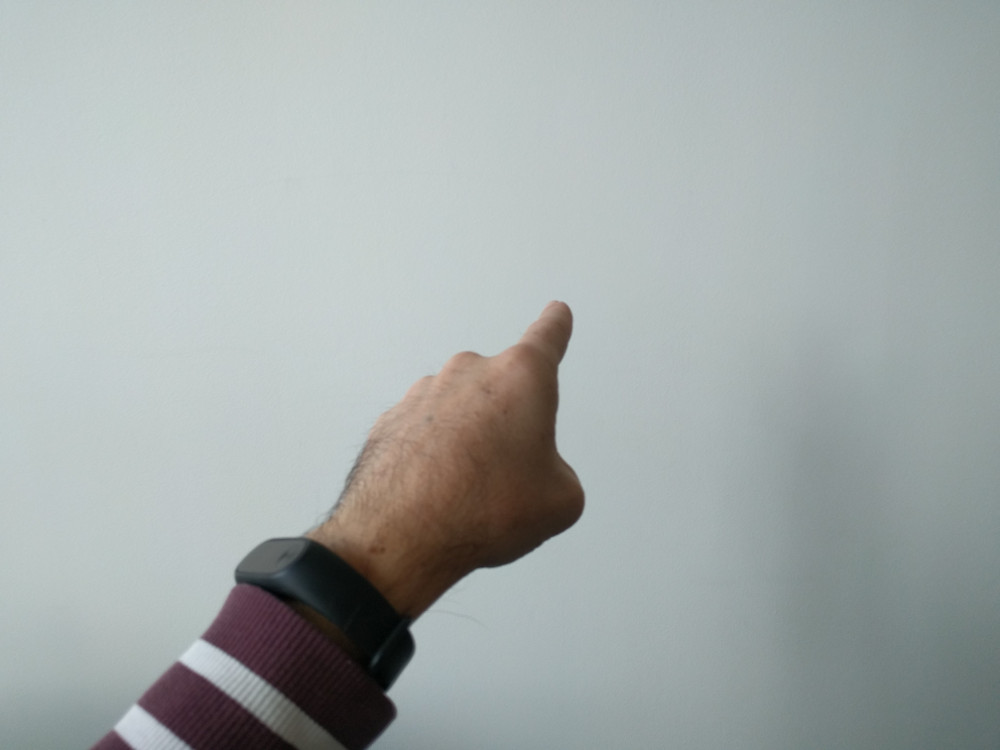
\includegraphics[width=0.95\linewidth]{figures/1.jpg}
   \end{minipage} 
   \begin{minipage}[c]{0.3\linewidth}
      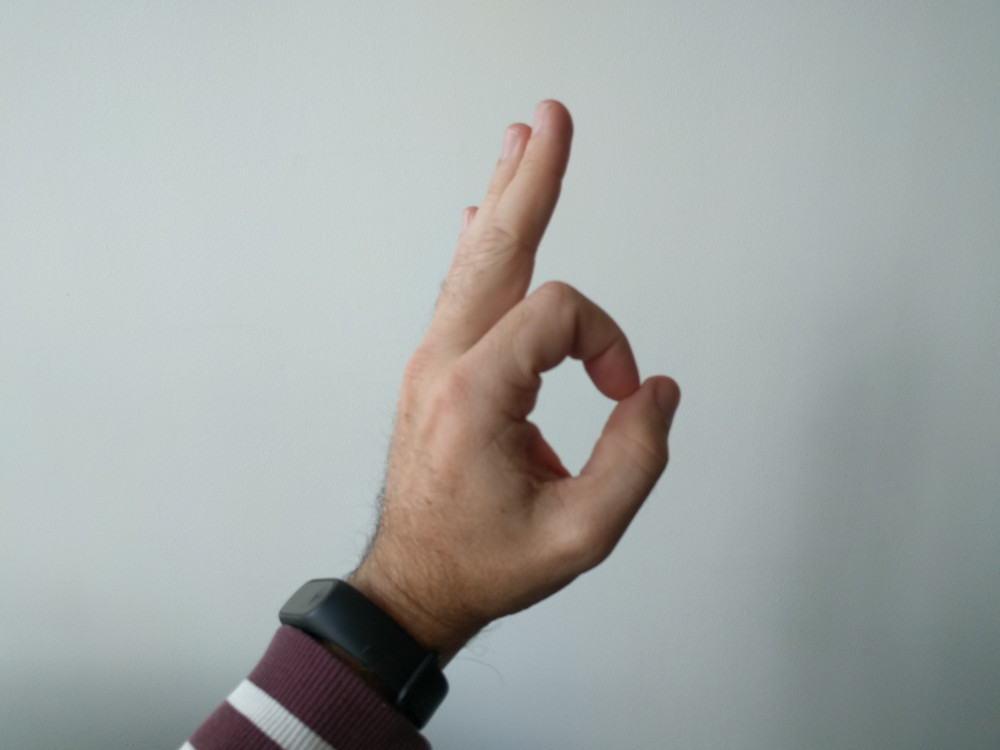
\includegraphics[width=0.95\linewidth]{figures/2.jpg}
   \end{minipage}
   \begin{minipage}[c]{0.3\linewidth}
      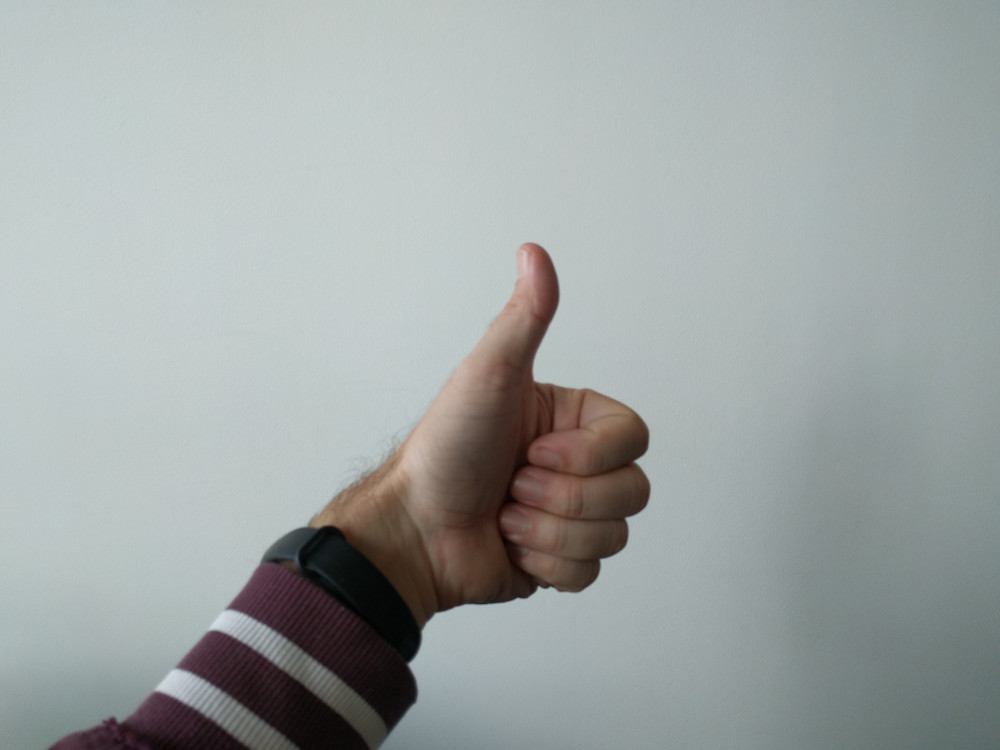
\includegraphics[width=0.95\linewidth]{figures/3.jpg}
   \end{minipage} \\
   \vspace{1em}
   \begin{minipage}[c]{0.3\linewidth}
      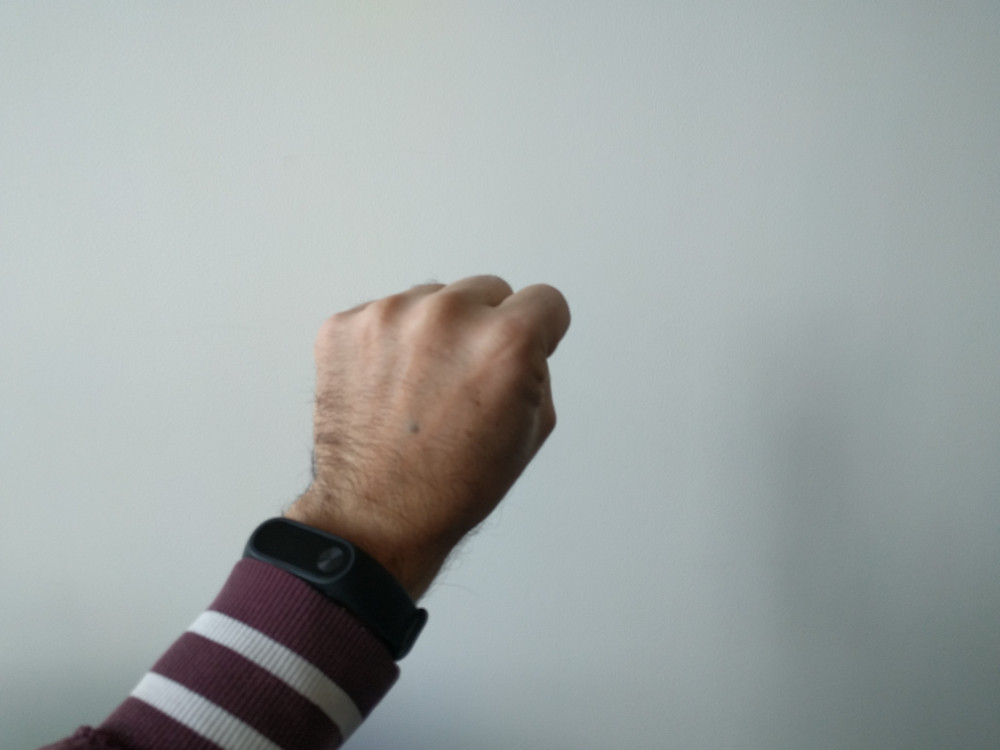
\includegraphics[width=0.95\linewidth]{figures/4.jpg}
   \end{minipage}   
   \begin{minipage}[c]{0.3\linewidth}
      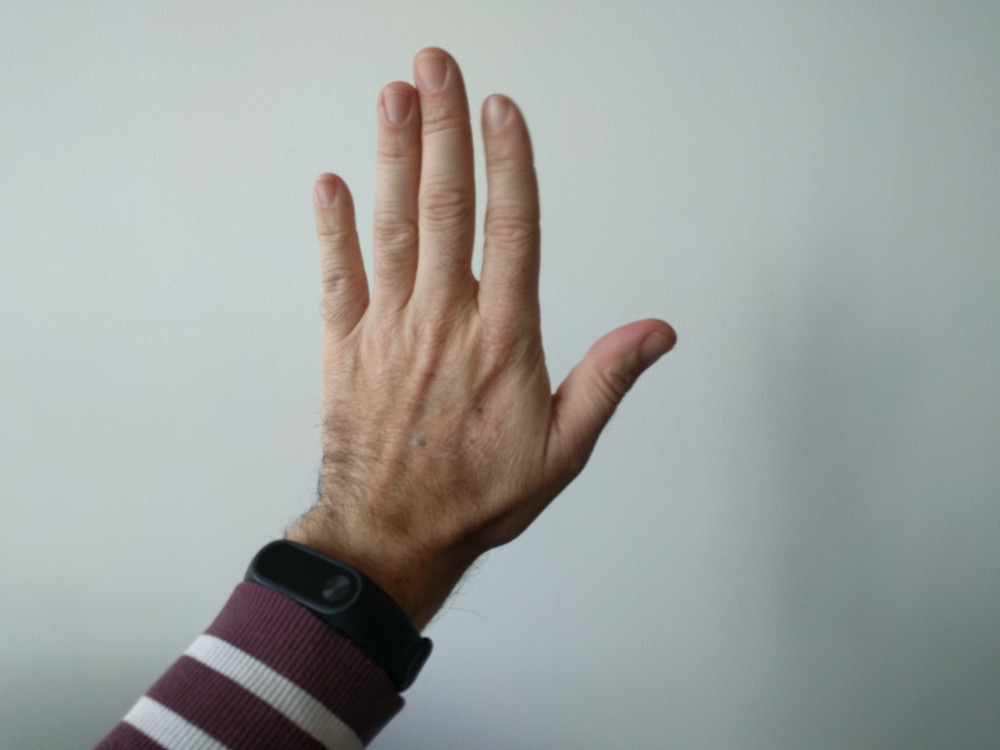
\includegraphics[width=0.95\linewidth]{figures/5.jpg}
   \end{minipage}   
   \caption{Les 5 gestes à reconnaître}
   \label{fig:gestures}
\end{figure}

Toutes les vidéos ont été réalisées en intérieur, avec des personnes marchant ou s'arrêtant aléatoirement.
Aucune consigne de positionnement n'ayant été donnée, pour permettre une grande disparité des gestes et de leur durée, des fonds, et des mouvement réalisés.
Les 29 heures de vidéos générée représentent 1669 différents gestes, ainsi que 1830 segments de vidéos sans gestes avec des fond similaire, pouvant être utilisés pour détecter les moments sans gestes.
La tableau~\ref{tab:videoGestes}, récapitule le nombre d'image pour chacuns des gestes.
Les segments de transition entre chaque geste contiennent généralement très peu d'images mais sont très nombreux, leur total étant de 23023 images.

\begin{table}
	\centering
	\caption{}
	\label{tab:videoGestes}
	\begin{tabular}{|l|c|}
		\hline
        			& \#Images \\
		\hline
        Total		& 120 055 \\
		\hline
        g1          & 8890  \\
        g2          & 8792  \\
        g3          & 9062  \\
        g4          & 9236  \\
        g5          & 8800  \\
        Sans main   & 52252 \\        
		\hline
        Transition	& 23023 \\
		\hline
	\end{tabular}
\caption{Nombres d’images pour chaque geste présent dans la collection}
\end{table}






\subsection{Gestes sur fond vert}


L'avantage de créer des vidéos de gestes devant un fond vert est le suivant: la segmentation de la main\/du bras à reconnaître dans l'image est entièrement automatisable; il est alors possible d'intégrer ultérieurement autant d'arrière-plans différents de l'image acquise que souhaité. 

\begin{figure}[htb]
\centering
   \begin{minipage}[c]{0.95\linewidth}
      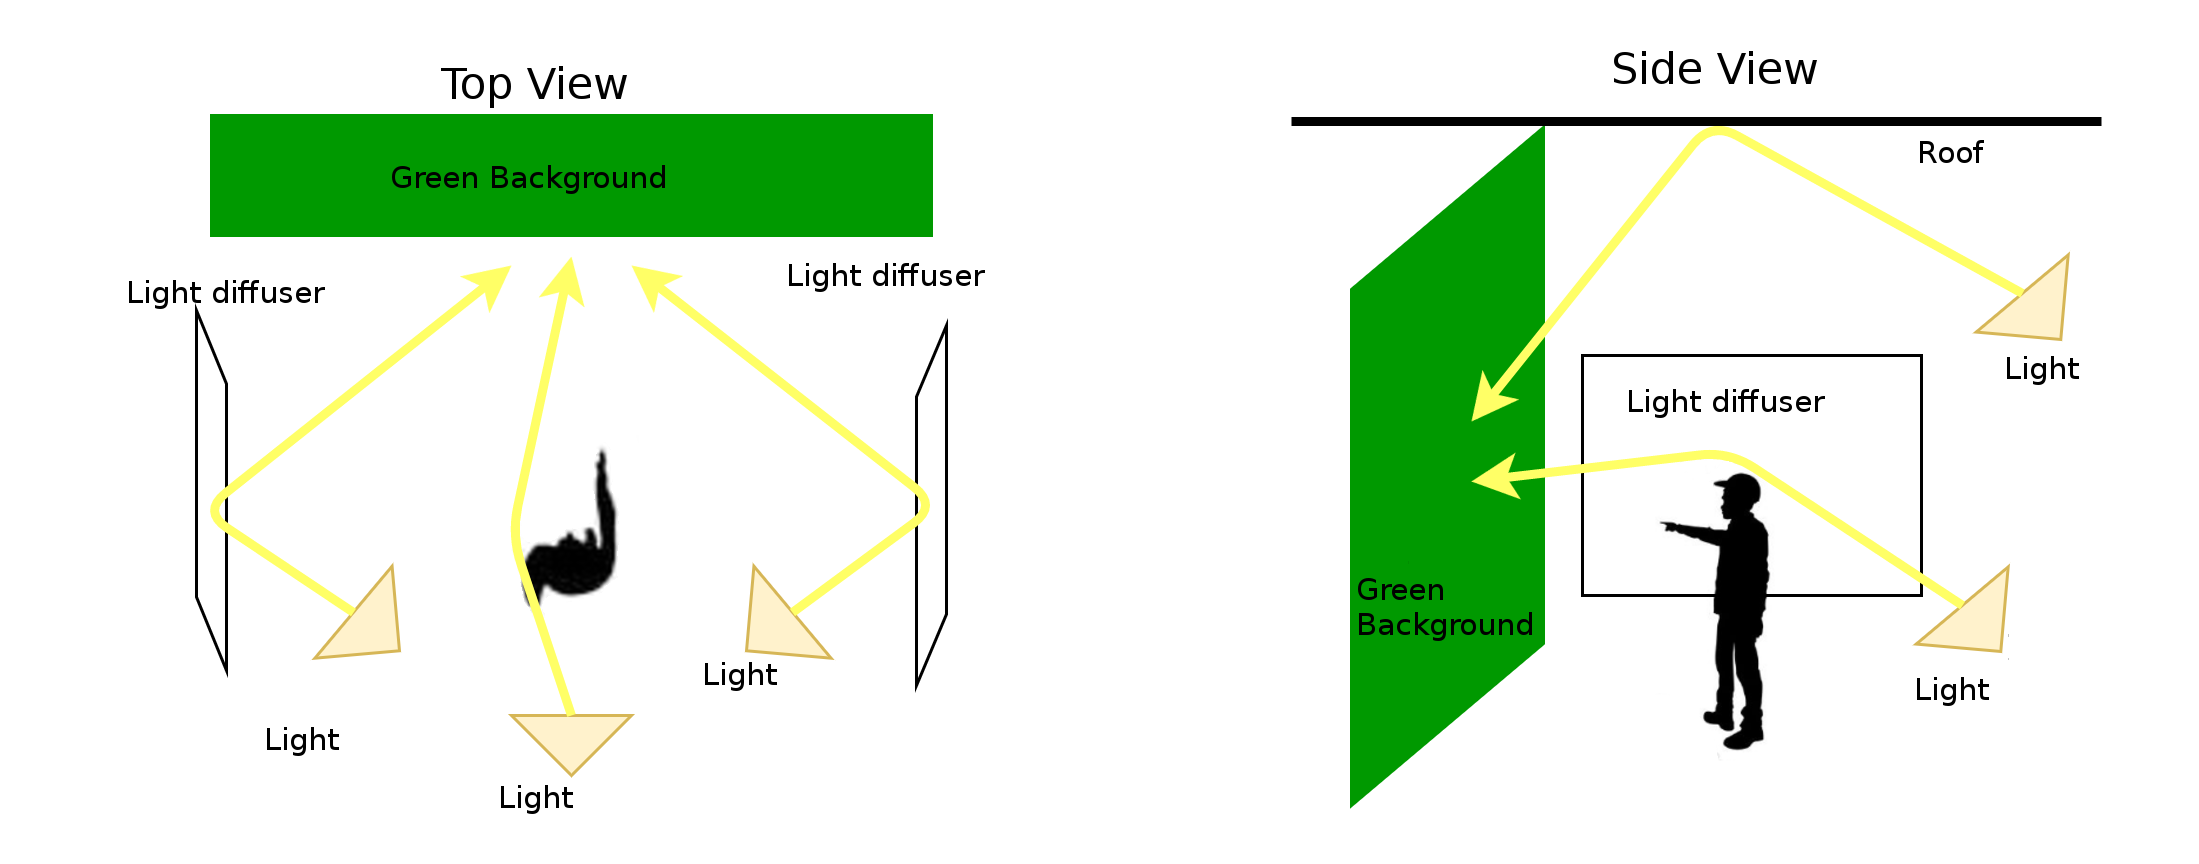
\includegraphics[width=0.95\linewidth]{figures/FondVertEN.png}
   \end{minipage} \\
   \vspace{1em}
   \begin{minipage}[c]{0.4\linewidth}
      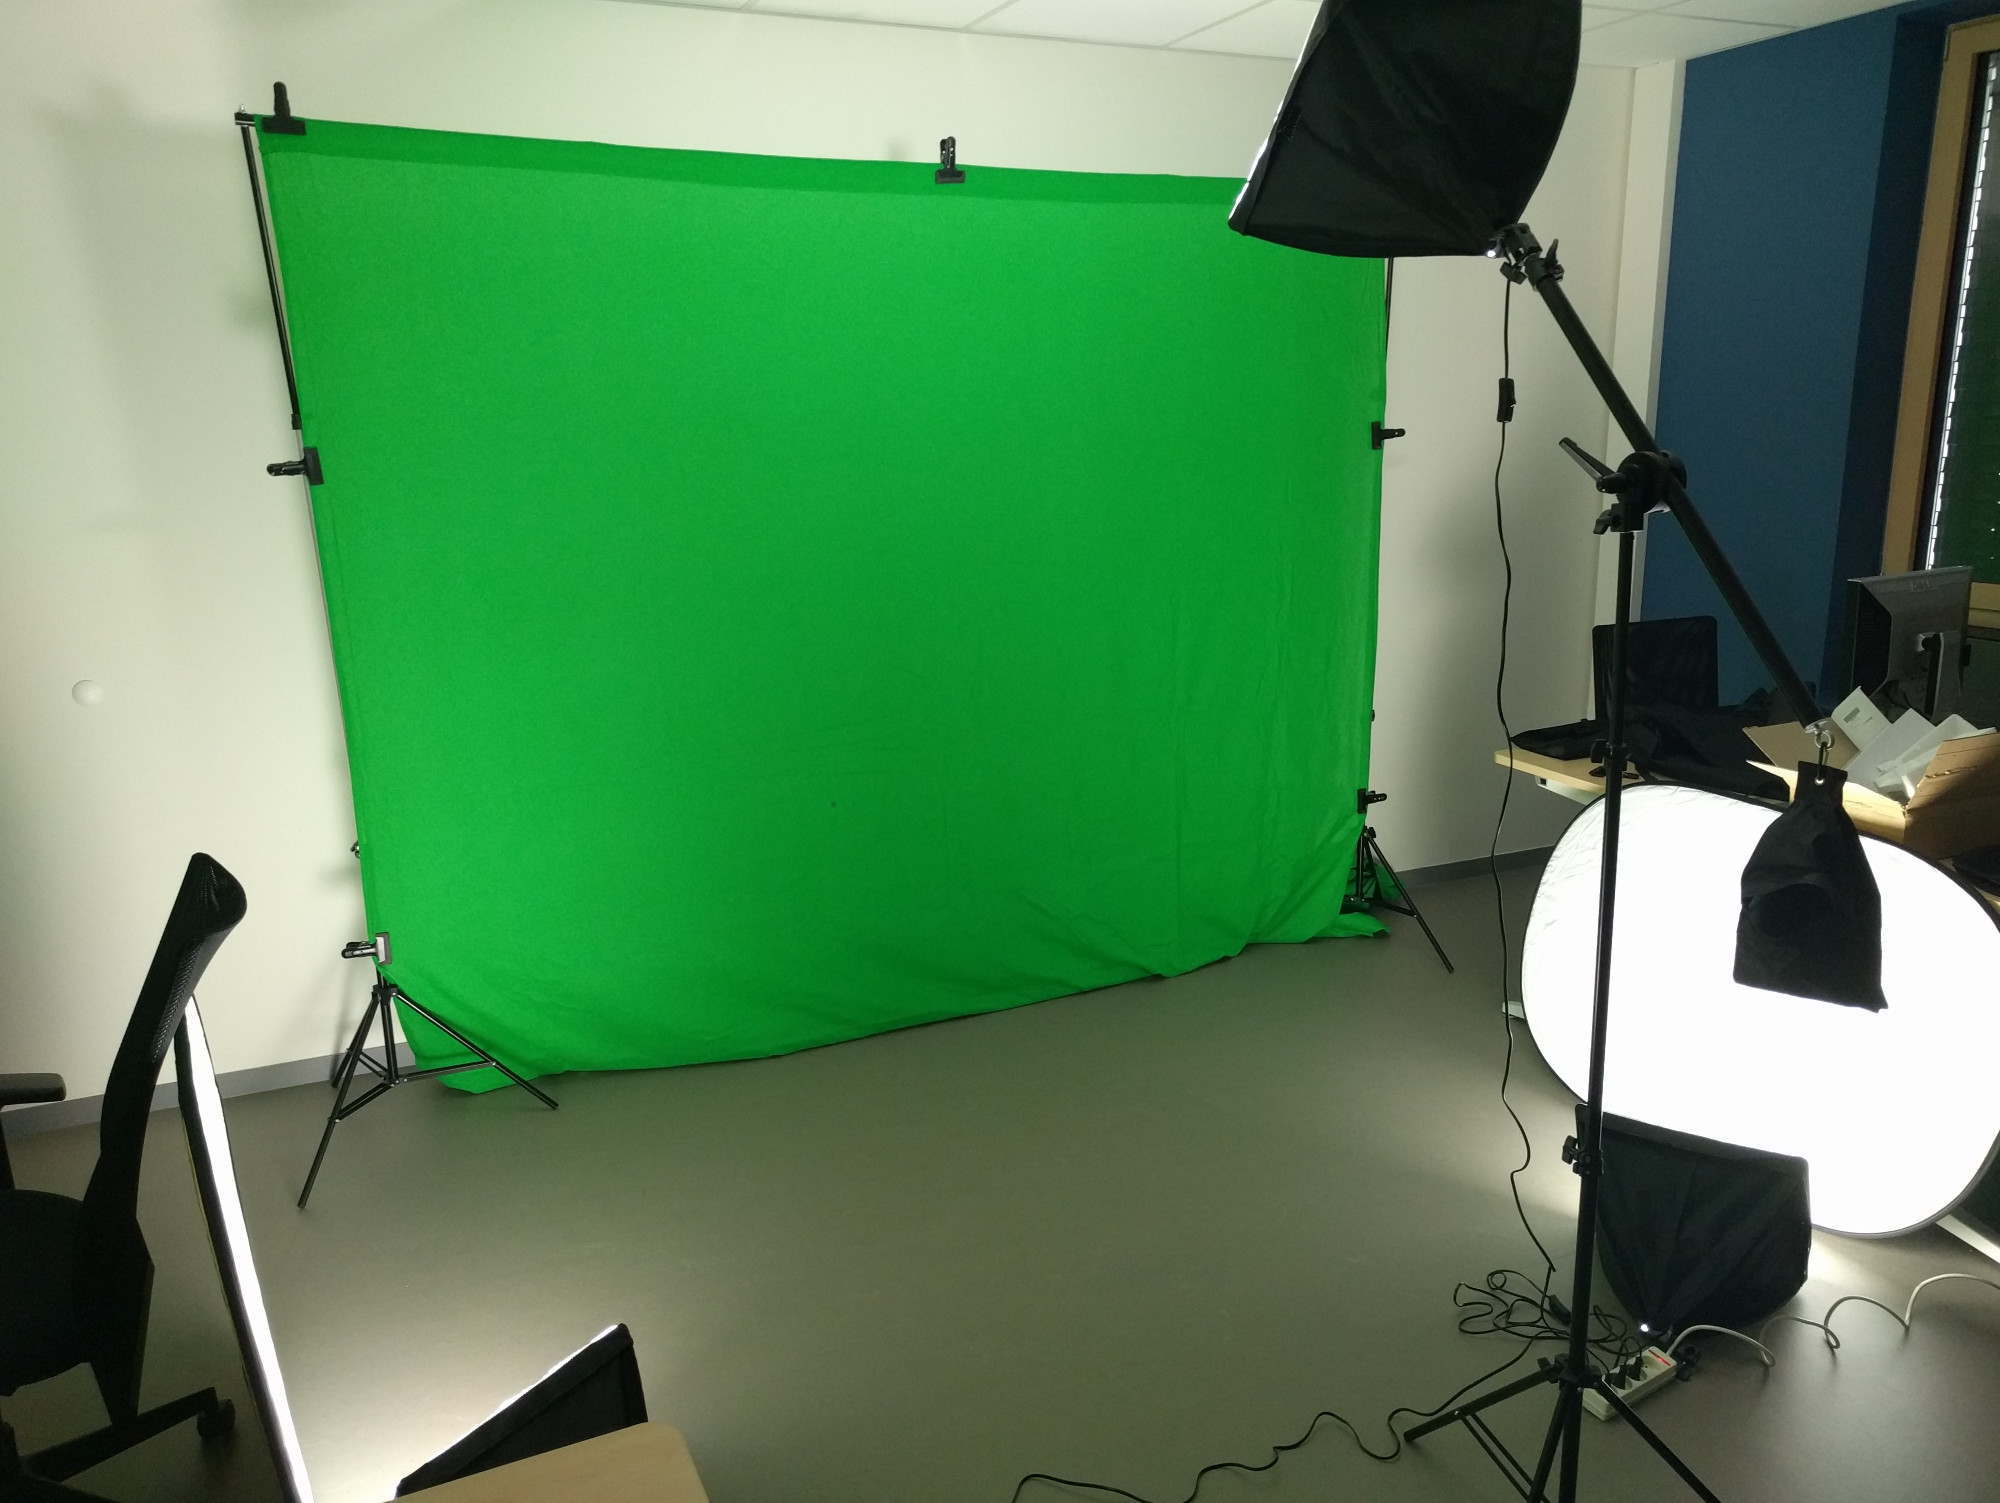
\includegraphics[width=0.95\linewidth]{figures/img1.jpg}
   \end{minipage}
   \begin{minipage}[c]{0.4\linewidth}
      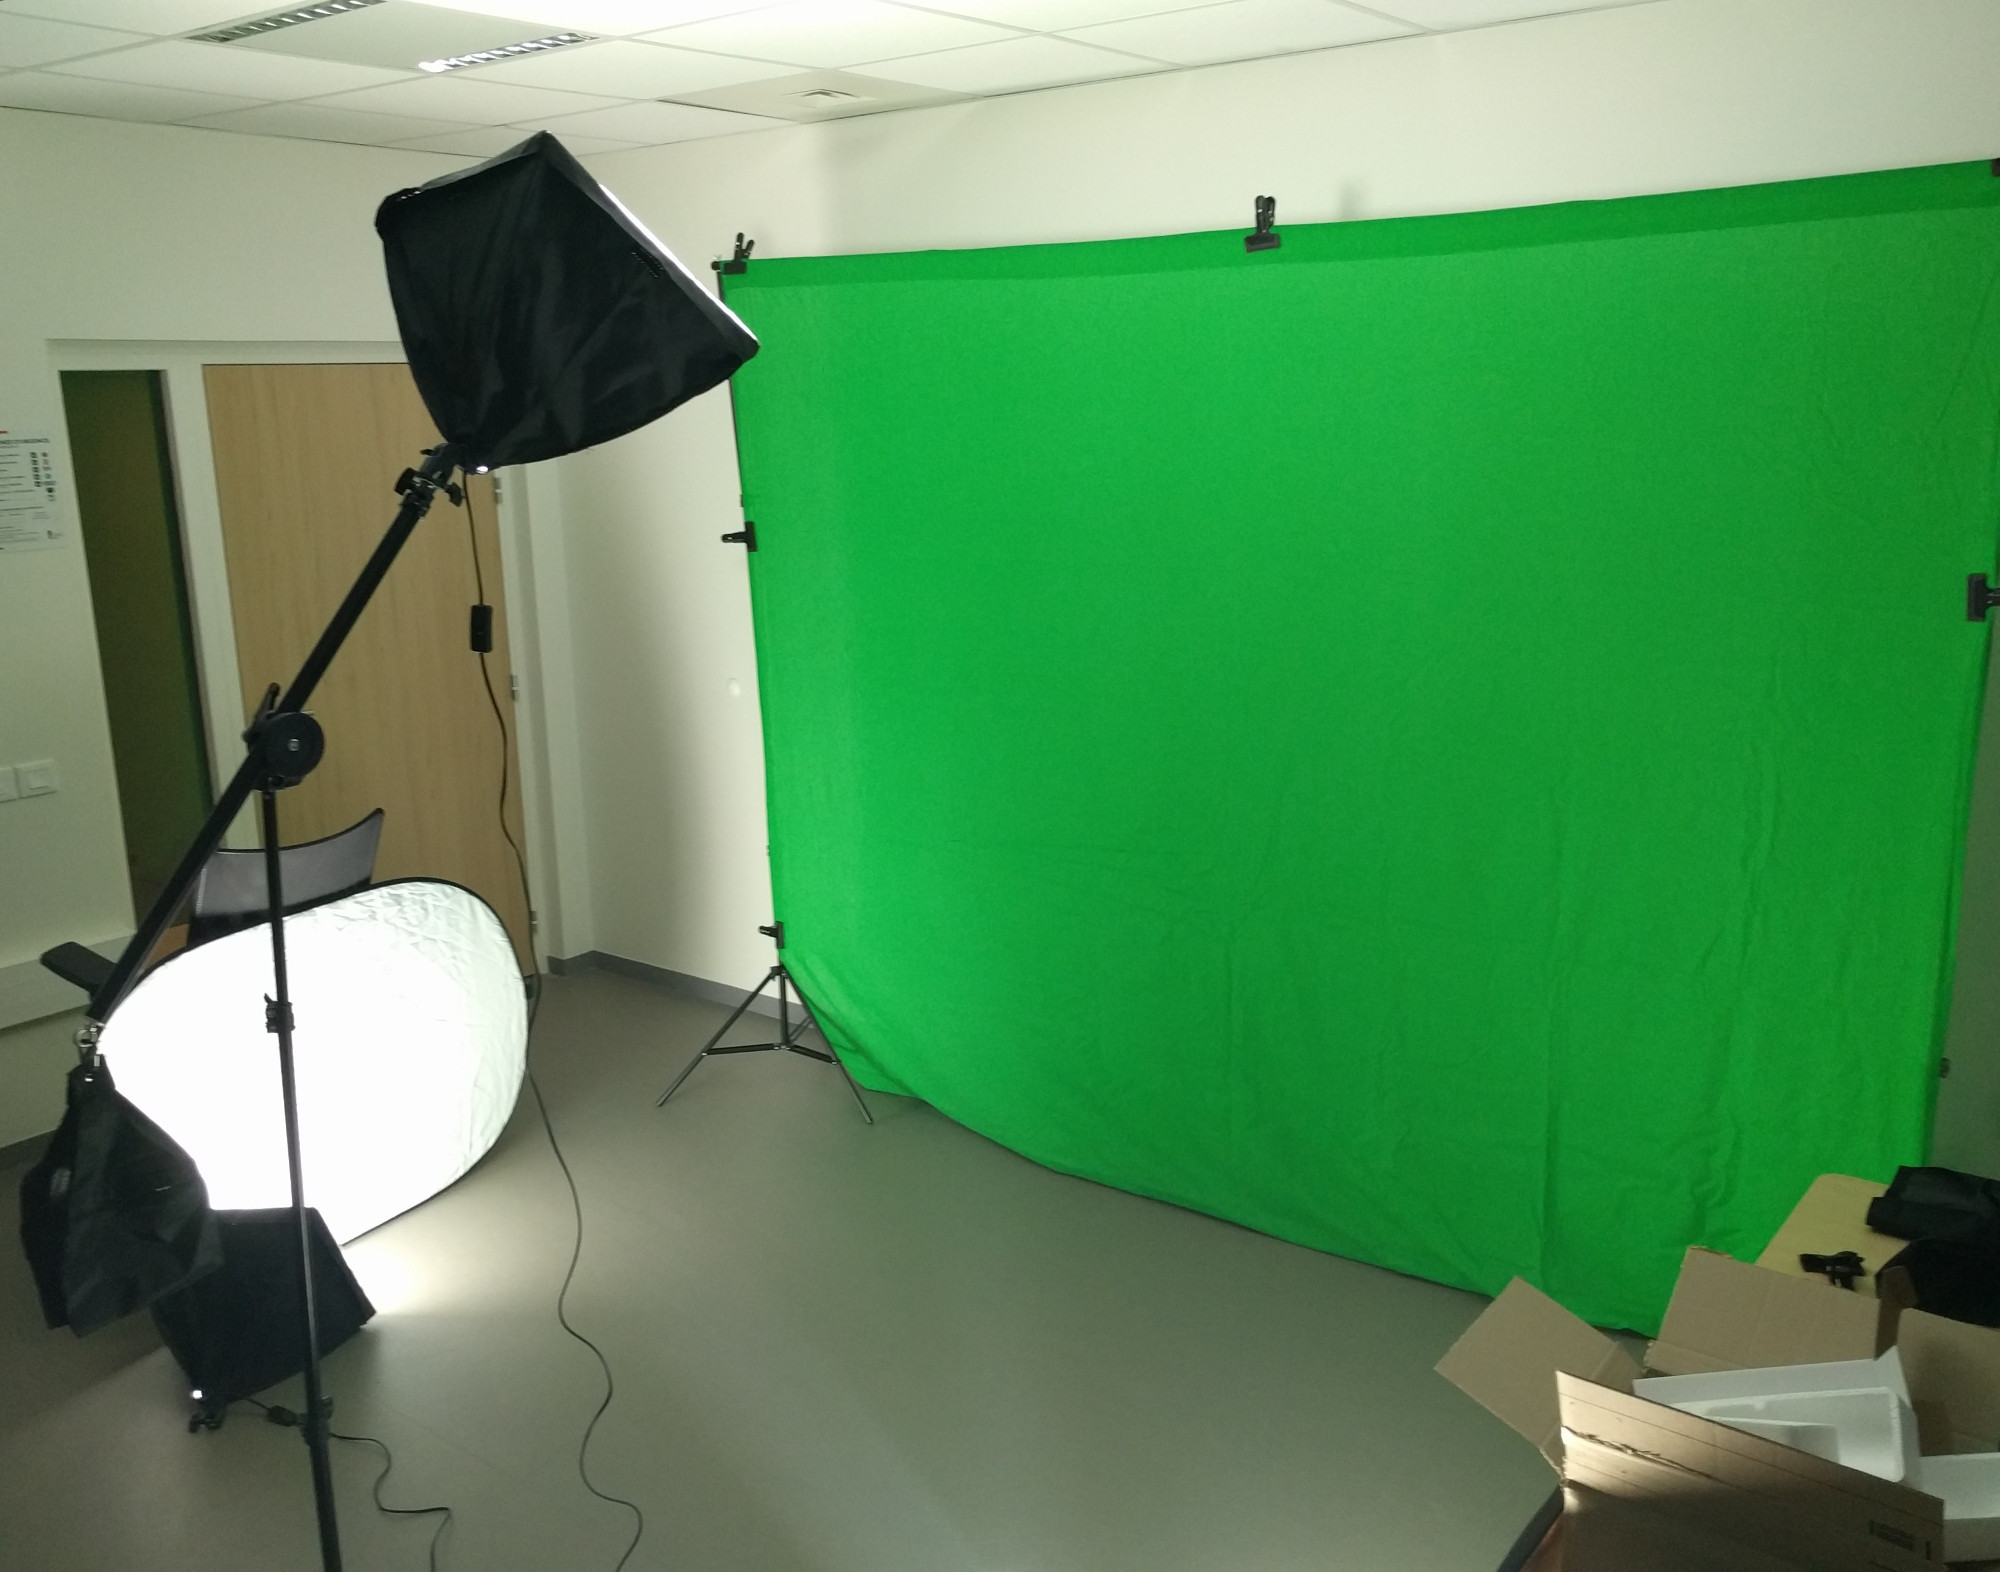
\includegraphics[width=0.95\linewidth]{figures/img2.jpg}
   \end{minipage}
   \caption{Installation du fond-vert (\url{www.videomaker.com})}
 \label{fig:FondVert}
\end{figure}

La figure~\ref{fig:FondVert} présente l'installation utilisée pour produire le corpus. Le matériel nécessaire (un fond vert sur la structure amovible, 3 lumières et 2 réflecteurs) est facilement disponible et peu coûteux.

Pour capturer une vidéo d'apprentissage des données, le processus est le suivant: une personne est équipée d'une caméra qui filme devant la personne (smartphone ou caméra positionné sur la poitrine). La personne est placée face à un fond vert où l'éclairage est contrôlé pour éviter les ombres sur l'écran (2 lumières de chaque côté dirigées vers des diffuseurs qui sont dirigés vers le fond vert, une lumière sur la personne orientée vers le plafond). La personne effectue la série de gestes requise dans un ordre spécifique.




Dix personnes ont participé à la création de cette partie du corpus. Ils ont chacun fait 5 fois chaque geste avec les deux mains, ce qui correspond à 50 gestes par personne, 500 gestes au total. Dans la figure~\ref{fig:g1m}, on peut voir que les participants n'ont pas effectué les gestes de la même manière. Pour plus de généralité, nous laissons les gens libres d'effectuer les gestes à leur manière.


\begin{figure}[htb]
   \centering
   \begin{minipage}[c]{0.19\linewidth}
      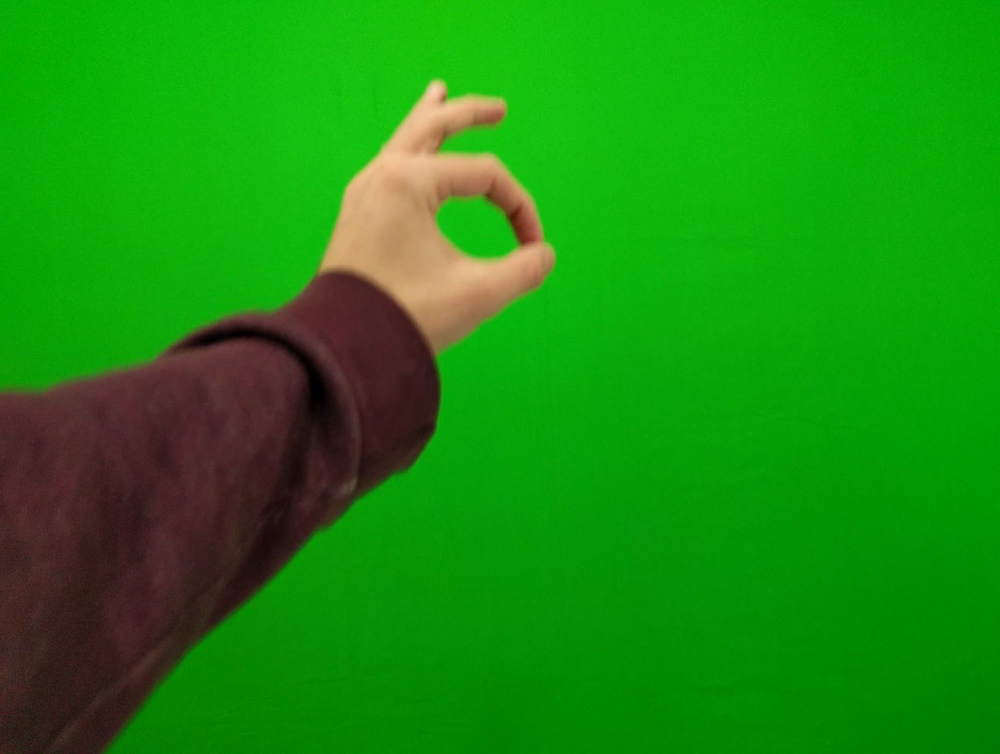
\includegraphics[width=0.95\linewidth]{figures/g2-1.jpg}
   \end{minipage} 
   \begin{minipage}[c]{0.19\linewidth}
      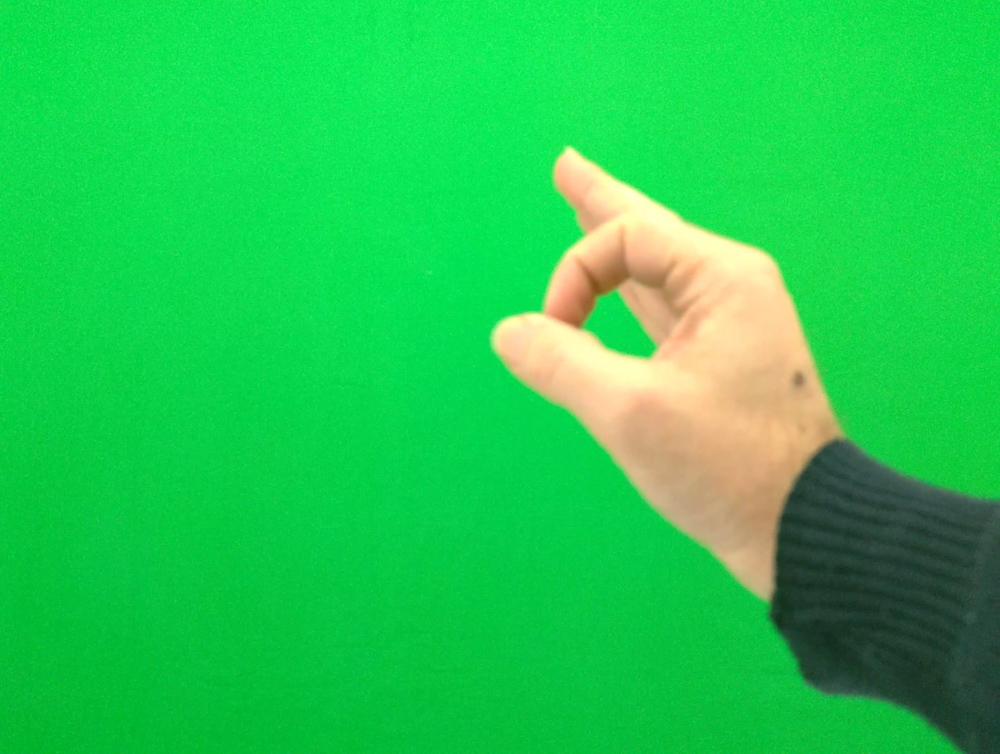
\includegraphics[width=0.95\linewidth]{figures/g2-3.jpg}
   \end{minipage}
   \begin{minipage}[c]{0.19\linewidth}
      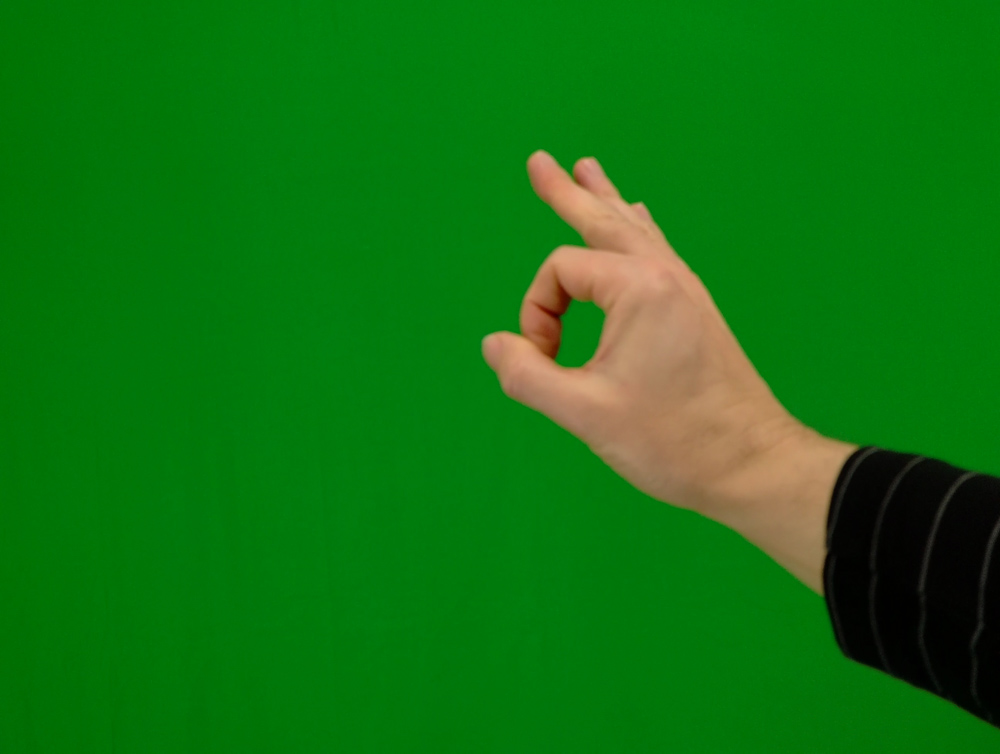
\includegraphics[width=0.95\linewidth]{figures/g2-5.jpg}
   \end{minipage} 
   \begin{minipage}[c]{0.19\linewidth}
      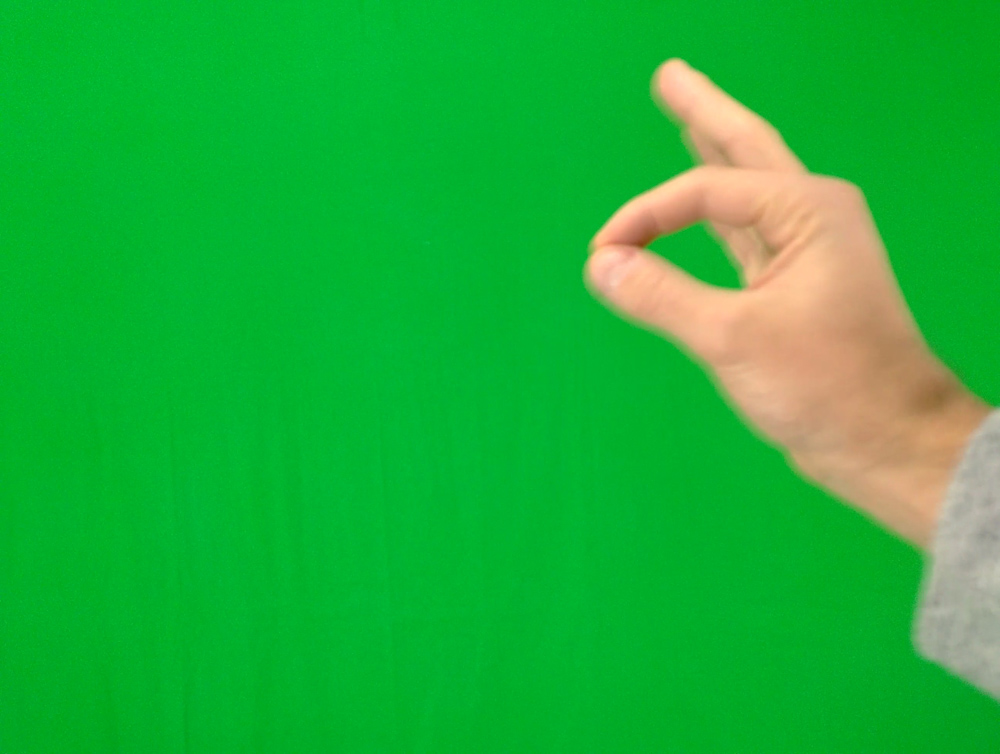
\includegraphics[width=0.95\linewidth]{figures/g2-7.jpg}
   \end{minipage} 
   \begin{minipage}[c]{0.19\linewidth}
      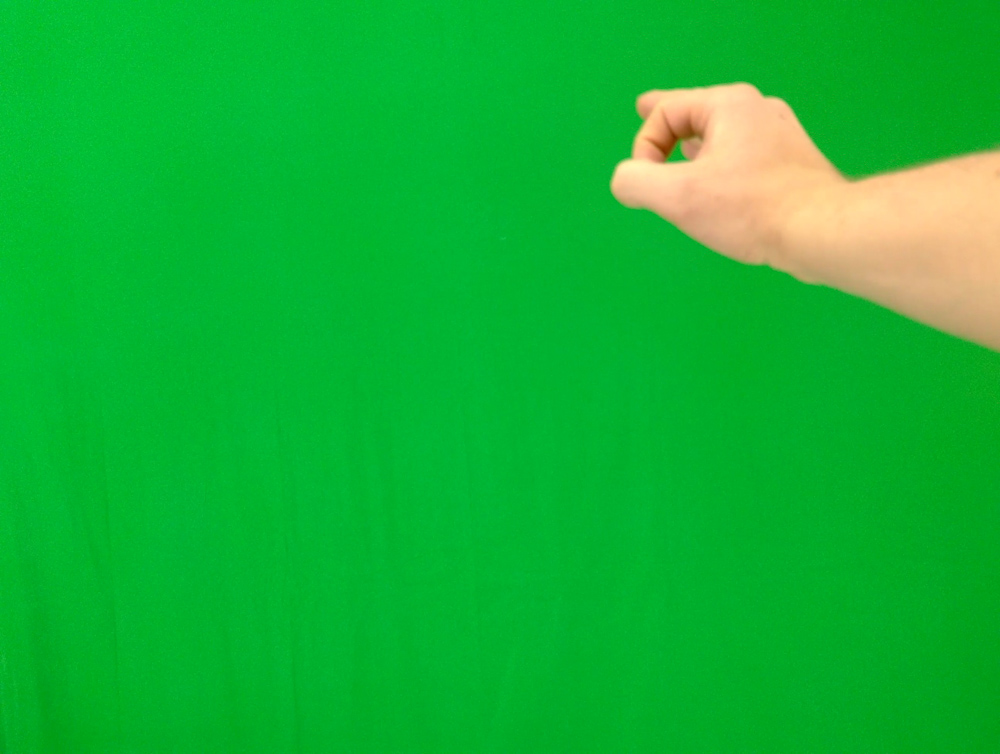
\includegraphics[width=0.95\linewidth]{figures/g2-9.jpg}
   \end{minipage}  \\      
   \vspace{1em}
   \begin{minipage}[c]{0.19\linewidth}
      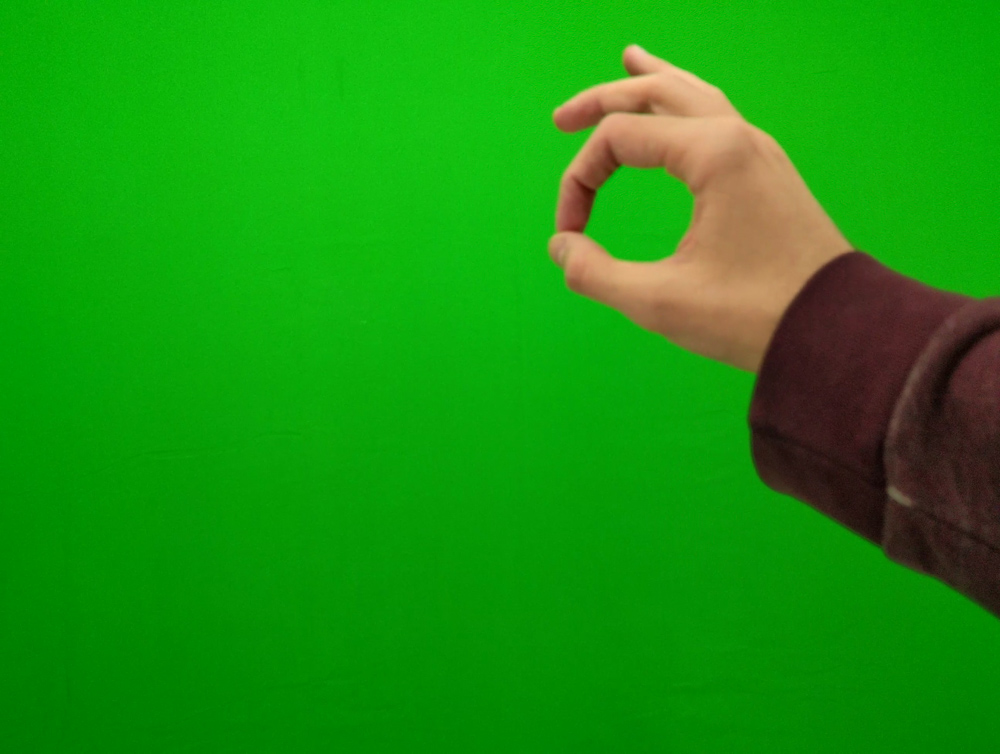
\includegraphics[width=0.95\linewidth]{figures/g2-2.jpg}
   \end{minipage} 
   \begin{minipage}[c]{0.19\linewidth}
      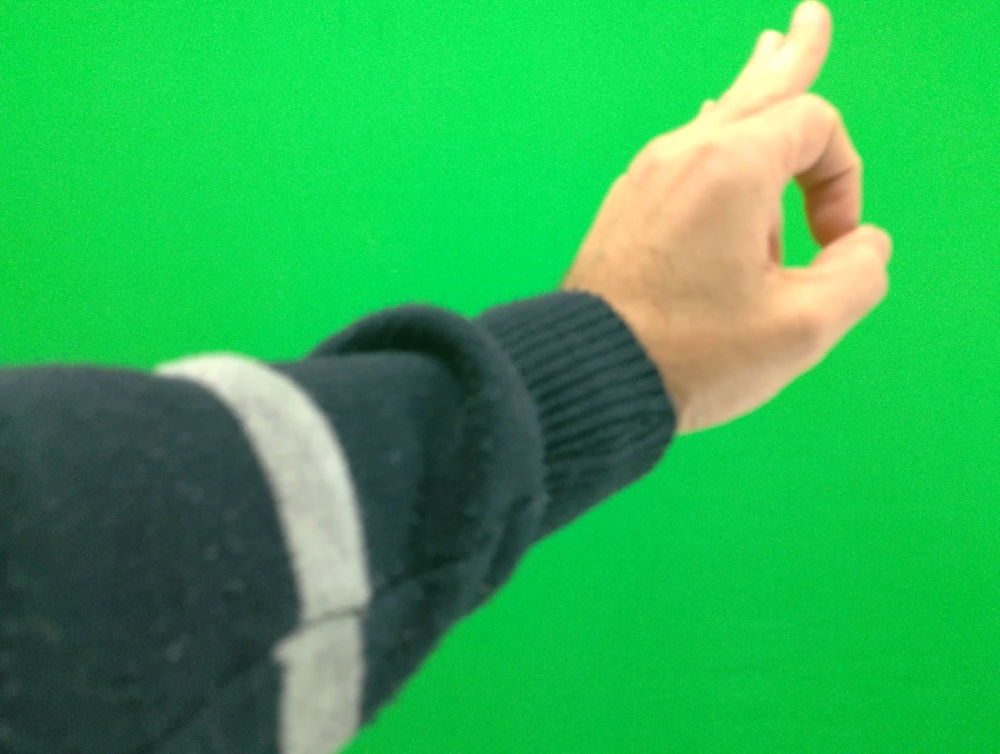
\includegraphics[width=0.95\linewidth]{figures/g2-4.jpg}
   \end{minipage} 
   \begin{minipage}[c]{0.19\linewidth}
      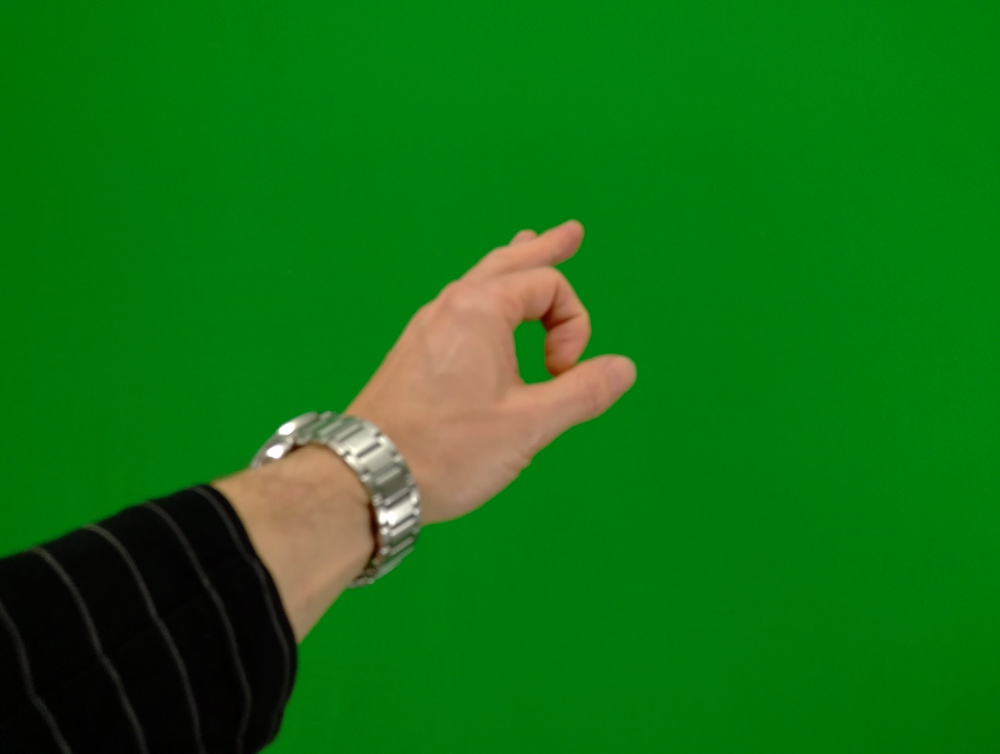
\includegraphics[width=0.95\linewidth]{figures/g2-6.jpg}
   \end{minipage} 
   \begin{minipage}[c]{0.19\linewidth}
      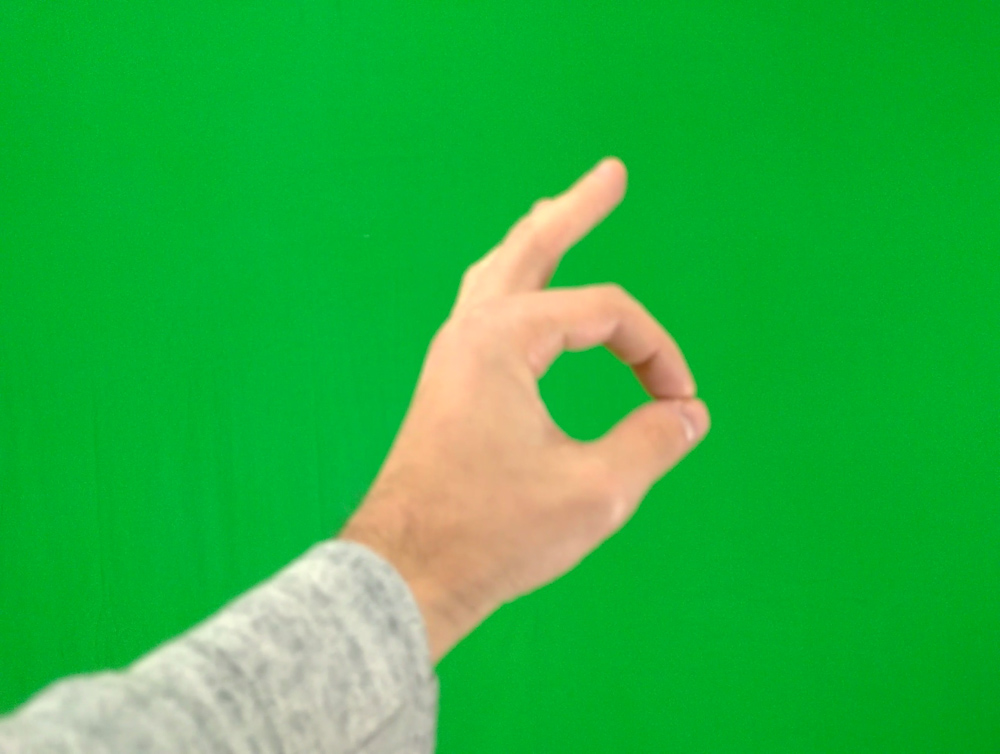
\includegraphics[width=0.95\linewidth]{figures/g2-8.jpg}
   \end{minipage} 
   \begin{minipage}[c]{0.19\linewidth}
      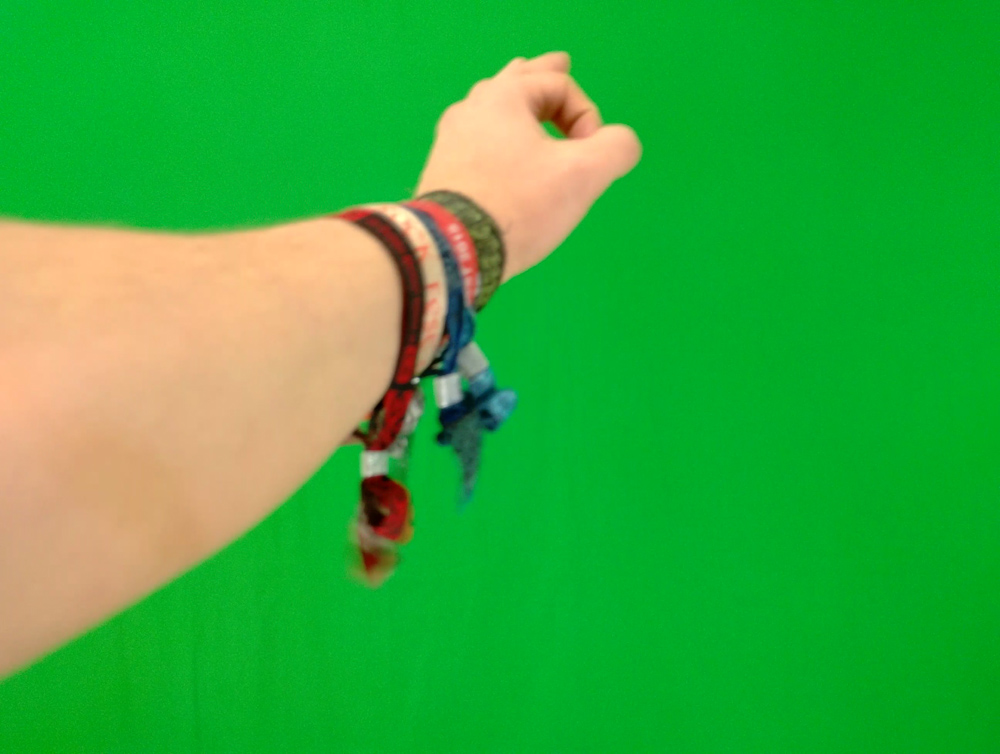
\includegraphics[width=0.95\linewidth]{figures/g2-10.jpg}
   \end{minipage} \\      
   \vspace{1em}
   \begin{minipage}[c]{0.19\linewidth}
      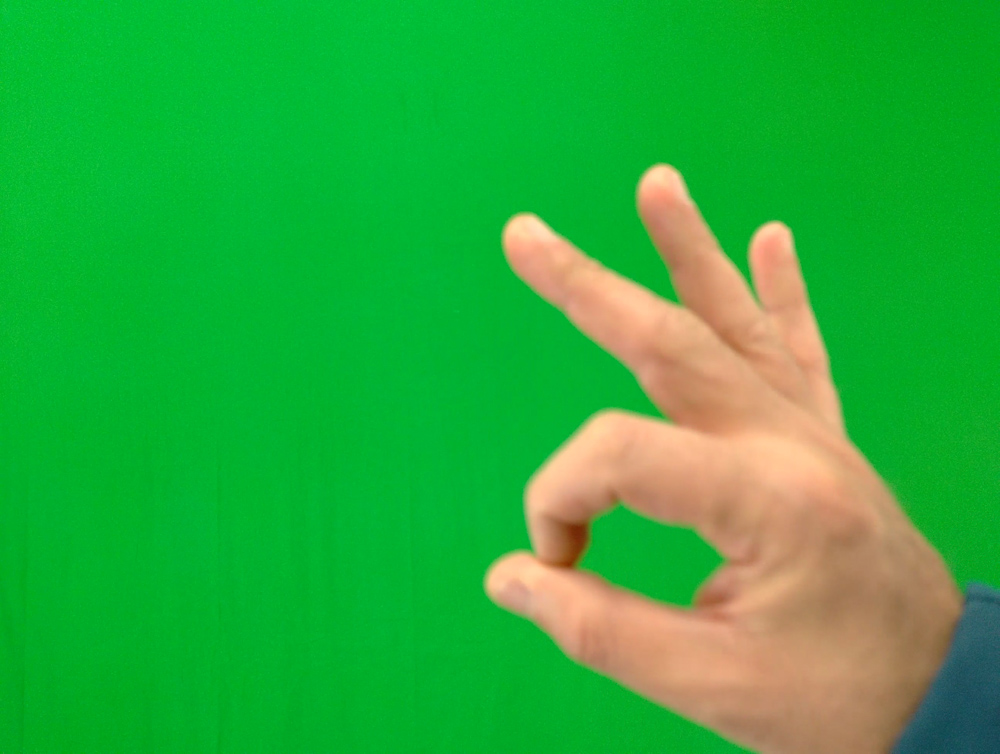
\includegraphics[width=0.95\linewidth]{figures/g2-11.jpg}
   \end{minipage} 
   \begin{minipage}[c]{0.19\linewidth}
      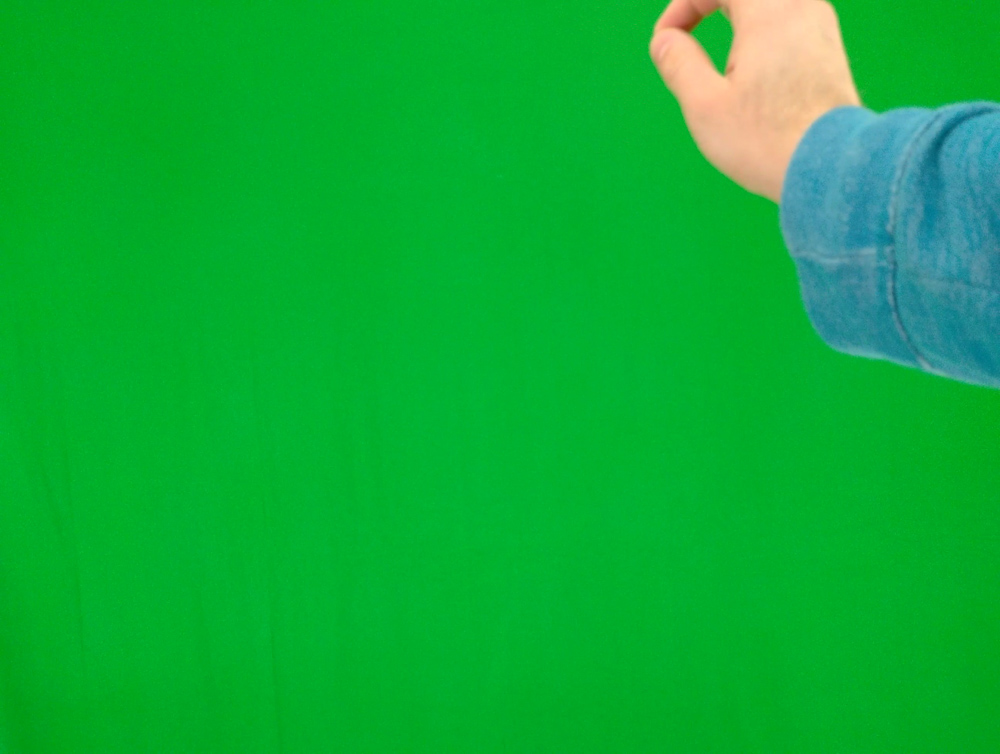
\includegraphics[width=0.95\linewidth]{figures/g2-13.jpg}
   \end{minipage}
   \begin{minipage}[c]{0.19\linewidth}
      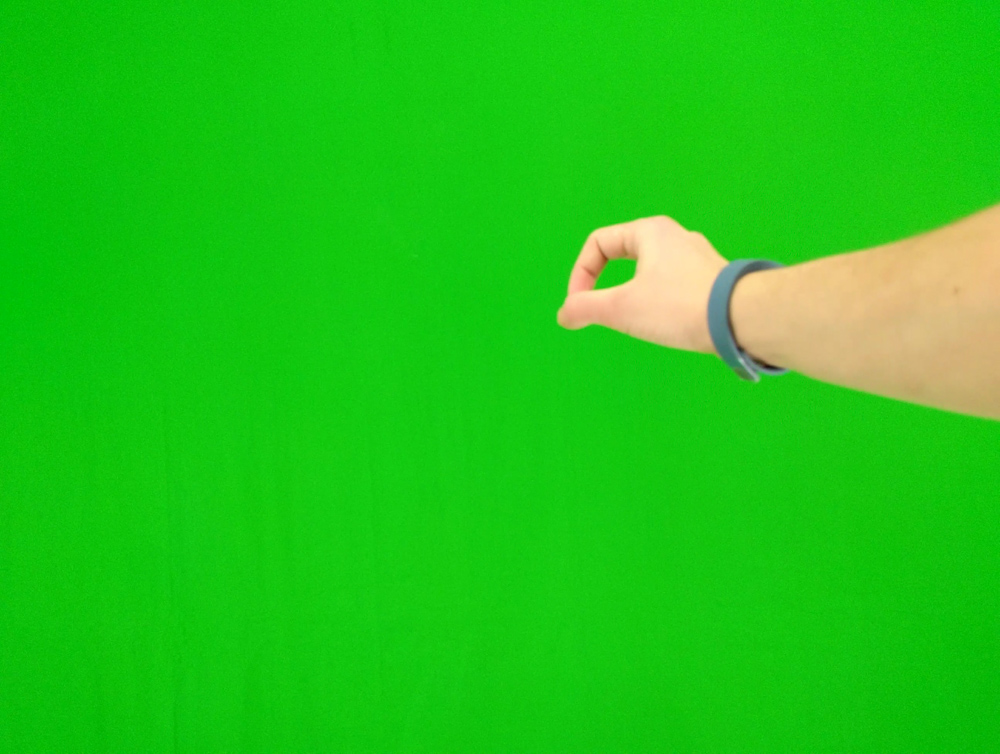
\includegraphics[width=0.95\linewidth]{figures/g2-15.jpg}
   \end{minipage} 
   \begin{minipage}[c]{0.19\linewidth}
      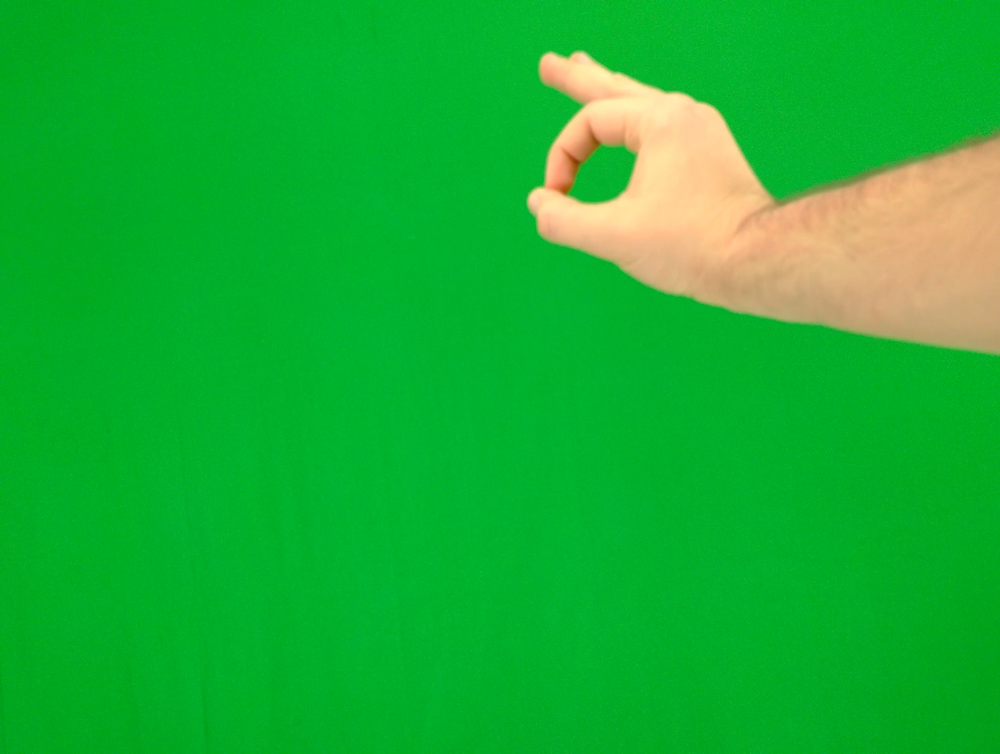
\includegraphics[width=0.95\linewidth]{figures/g2-17.jpg}
   \end{minipage} 
   \begin{minipage}[c]{0.19\linewidth}
      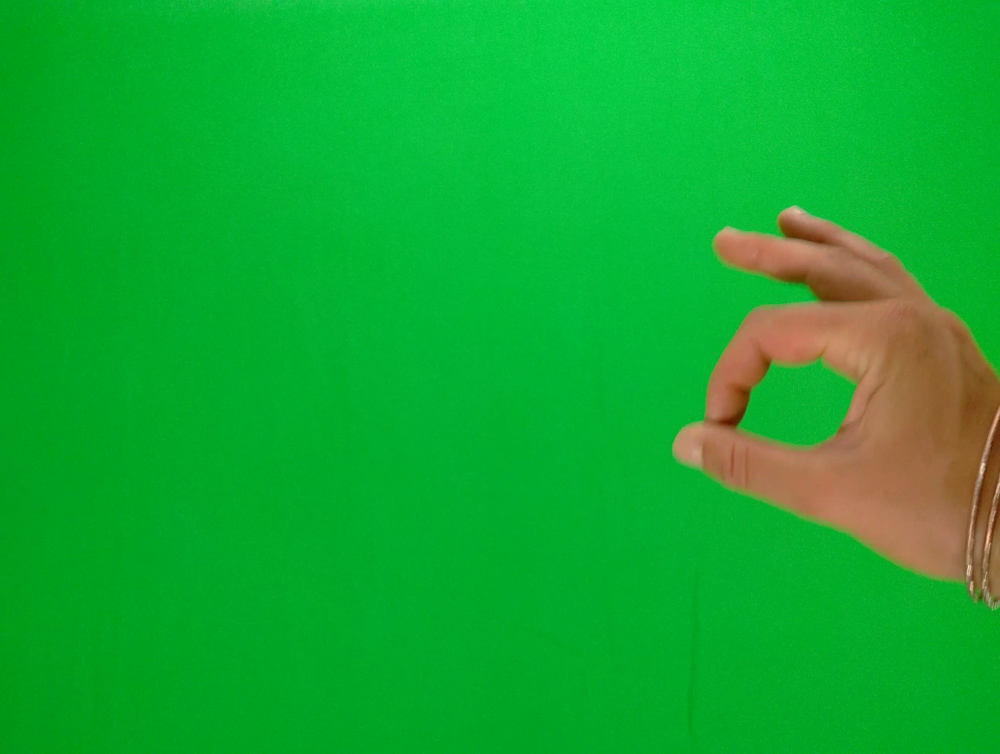
\includegraphics[width=0.95\linewidth]{figures/g2-19.jpg}
   \end{minipage}  \\      
   \vspace{1em}
   \begin{minipage}[c]{0.19\linewidth}
      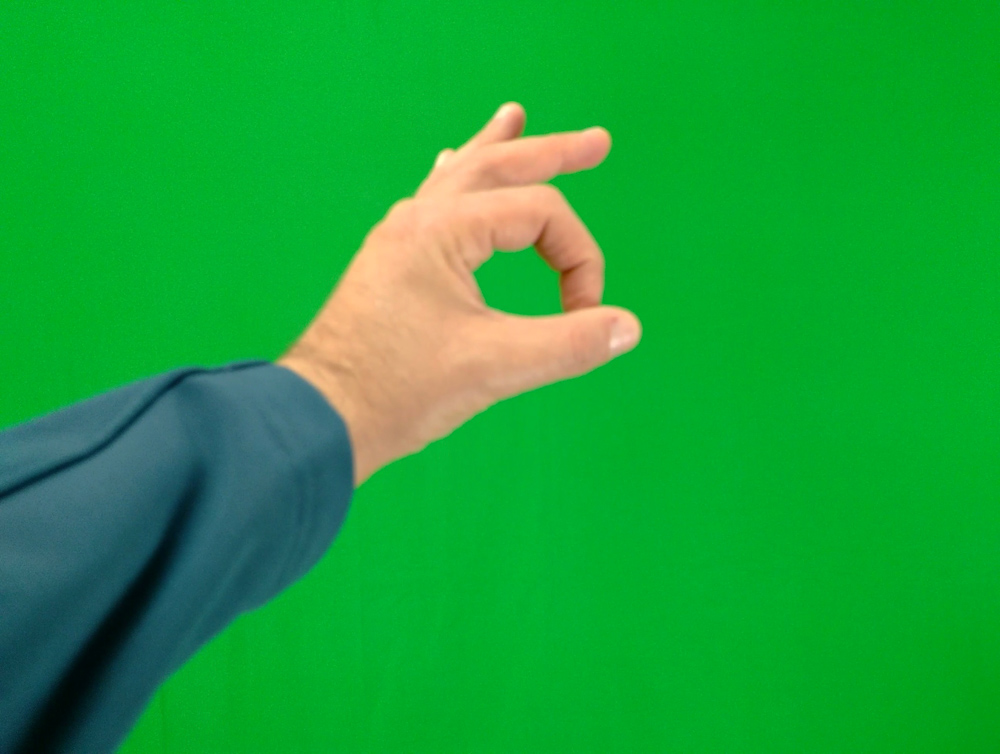
\includegraphics[width=0.95\linewidth]{figures/g2-12.jpg}
   \end{minipage} 
   \begin{minipage}[c]{0.19\linewidth}
      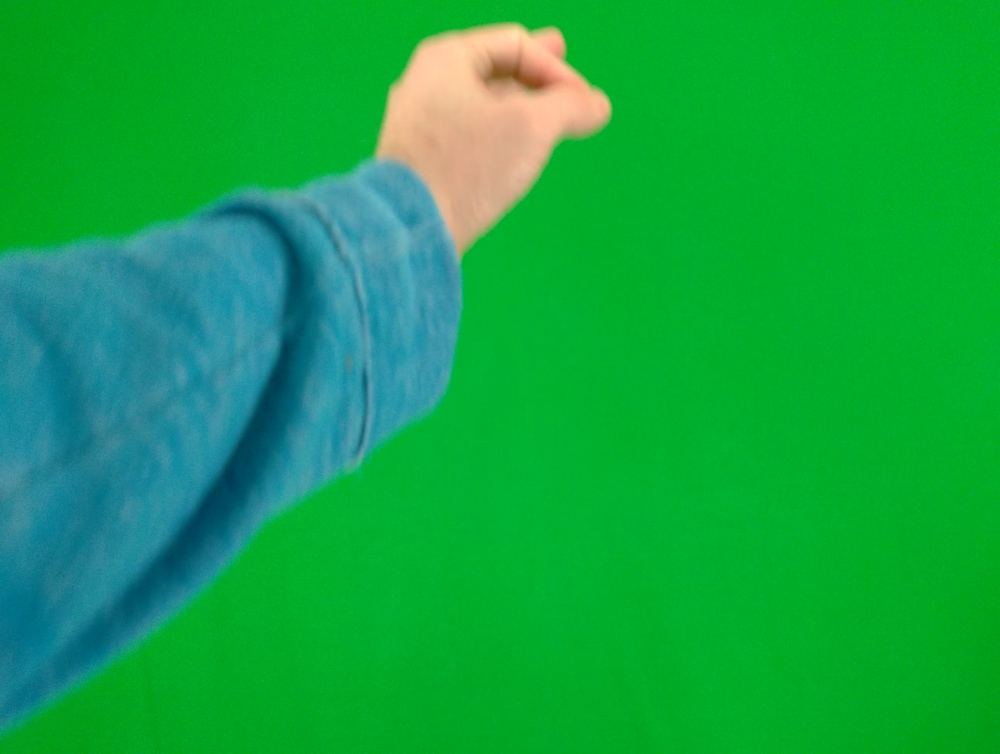
\includegraphics[width=0.95\linewidth]{figures/g2-14.jpg}
   \end{minipage} 
   \begin{minipage}[c]{0.19\linewidth}
      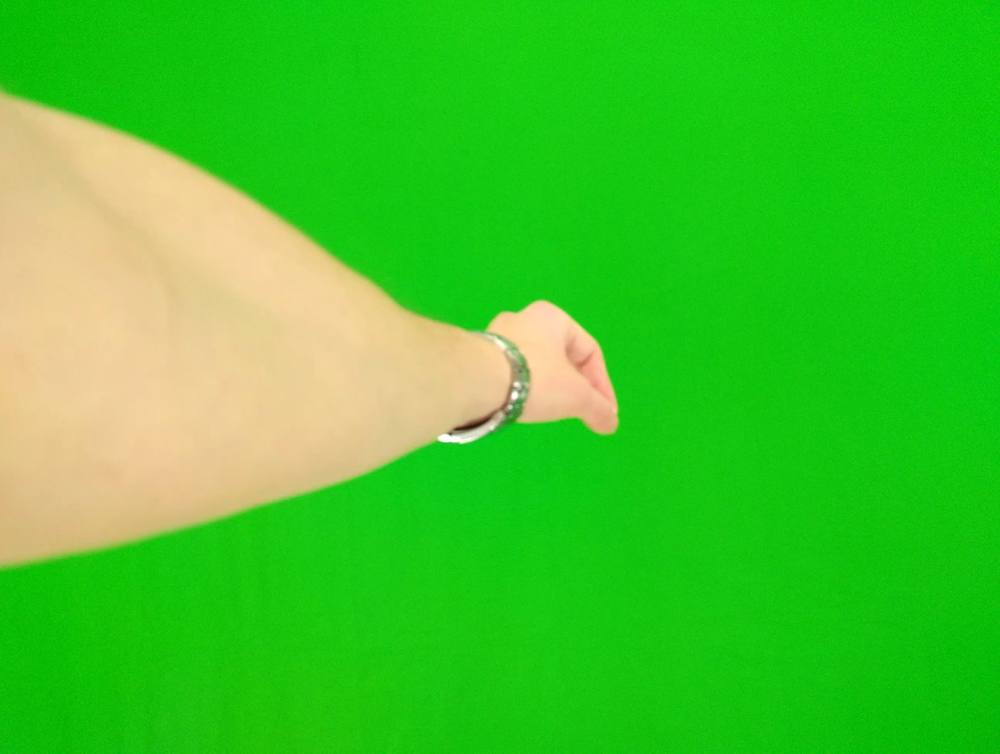
\includegraphics[width=0.95\linewidth]{figures/g2-16.jpg}
   \end{minipage} 
   \begin{minipage}[c]{0.19\linewidth}
      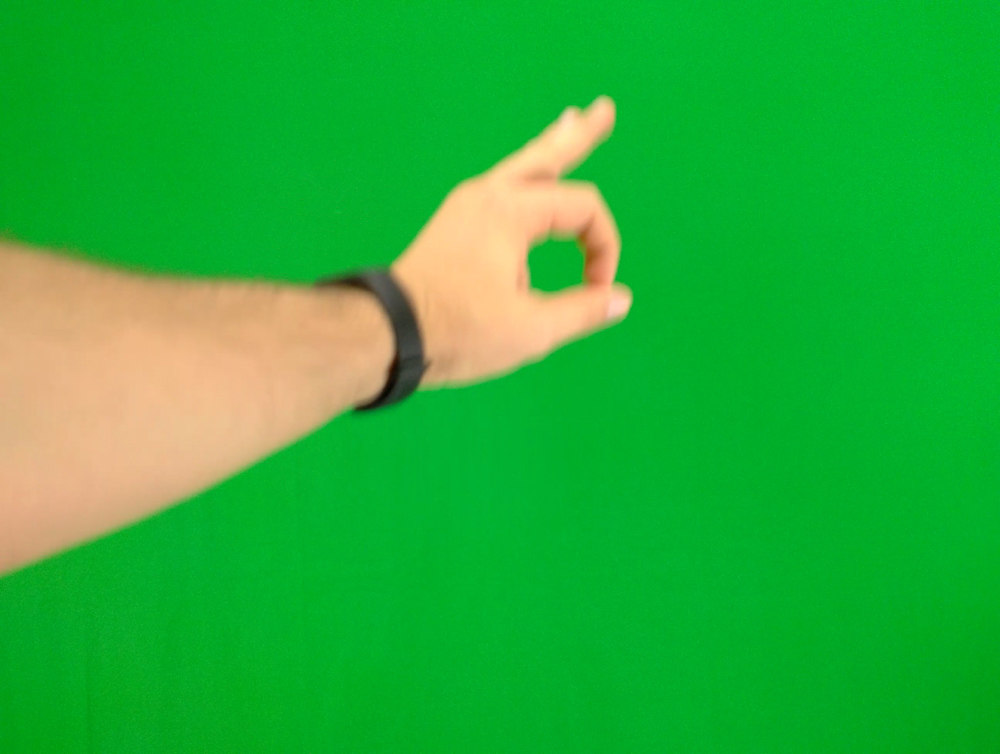
\includegraphics[width=0.95\linewidth]{figures/g2-18.jpg}
   \end{minipage} 
   \begin{minipage}[c]{0.19\linewidth}
      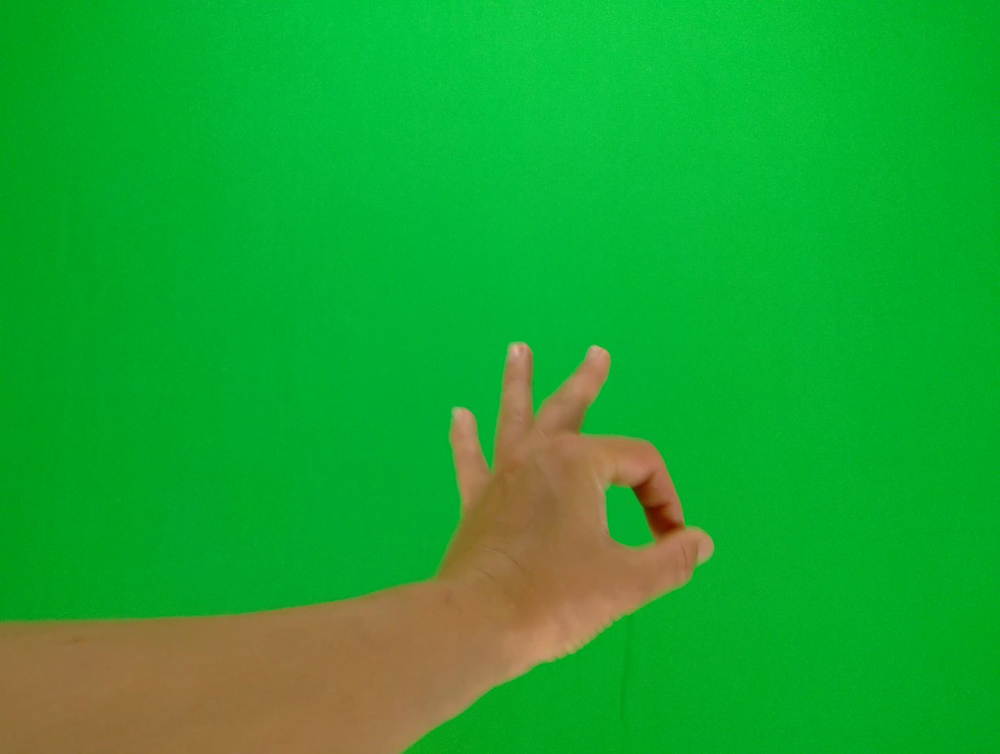
\includegraphics[width=0.95\linewidth]{figures/g2-20.jpg}
   \end{minipage} 
   \caption{Le même geste fait par différentes personnes. Peu d'instructions ont été données pour l'apparence désirée du geste}
   \label{fig:g1m}
\end{figure}

A posteriori, les vidéos sont collectées et un algorithme supprime le fond vert. A partir du résultat, un masque est créé avec la main en blanc sur fond noir (voir figure~\ref{fig:g1in}.) Ce masque correspond à la vérité de la segmentation spatio-temporelle du geste. fait pour vérifier / corriger que l'ordre a été respecté et que l'algorithme de détection de mouvement n'a pas échoué (moins de cinq minutes pour cinquante gestes capturés).

\begin{figure}[htb]
	\centering
	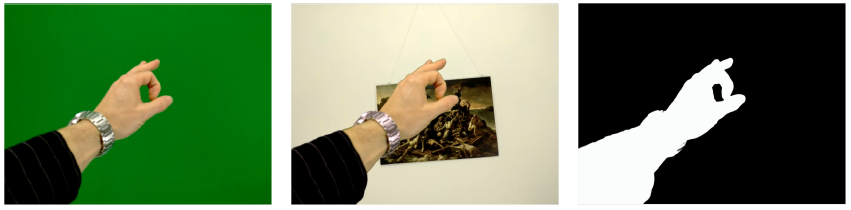
\includegraphics[width=1\linewidth]{figures/Capture4.PNG}
	\caption{Le geste capturé sur un fond vert, avec un arrière-plan intégré et la segmentation automatique}
	\label{fig:g1in}
\end{figure}

Cette solution, en plus d'obtenir une bonne segmentation automatique de la main en supprimant le fond vert, permet le changement de l'arrière-plan afin de générer de nouvelles données d'apprentissage à moindre coût tout en ayant déjà les annotations associées.







%%%%%%%%%%%%%%%%%%%%%%%%%%%%%%%%%%%%%%%%%%
%
%  Etude Geste
%
%%%%%%%%%%%%%%%%%%%%%%%%%%%%%%%%%%%%%%%%%%
\chapter{Etudes de la pertinence de l'interaction à base de geste}
\label{sec:etudeGestes}

Des séances de conception participatives ont été réalisées avec l'entreprise Multicom~\footnote{\url{http://www.multicom-ergonomie.com/}}.
L'objectif de ces séances était de réunir des utilisateurs potentiels du dispositif GUIMUTEIC, et de les faire s'entretenir sur les applications éventuelles, et l'interaction possible avec l'appareil.
Trois séances différentes ont été réalisées, avec chacune leurs objectifs séparés.

\section{Le dispositif proposé}

Ces séances ont pour but de réfléchir aux possibilités du dispositif GUIMUTEIC.
Ce qui est présenté aux participants est que l’appareil est constitué d’un casque audio, avec la possibilité d’un écran transparent, rabattable ou amovible.
Cette écran peut être sous la forme de lunette, ou de petit écran de coin de l’oeil.
Il peut également être équipé d’une surface tactile, sur l’écran ou sur un boîtier déporté.

Au niveau des applications, cette appareil est décrit comme une aide à la visite touristique, notamment dans le cadre des musées.
Les participants sont libre d’imaginer comment ce guide peut être utilisé, et quel est son objectif.

Ce dispositif n’est pas fixe, et les participants vont être amené à réfléchir aux améliorations possible.
Ce premier dispositif n’a pour but que de présenter une solution possible au projet GUIMUTEIC, aucune limite n’étant fixée aux participants quant à leurs idées.


\section{Les participants}

Dix participants ont été réunis pour ces séances.
Les profils ont été sélectionnés pour être varié, avec autant d'hommes que des femmes, des personnes actives, des étudiants ou des retraités, avec ou sans enfant.
La figure~\ref{fig:groupePersonnes} présente la répartition des participants en fonction de leurs habitudes de visite.
La majorité des participants n'ont jamais eu recours à un guide pour une visite organisée, et on voit une répartition équitable entre les personnes visitant les musées seuls ou en groupes.


\begin{figure}
\centering
\begin{minipage}[c]{.49\linewidth}
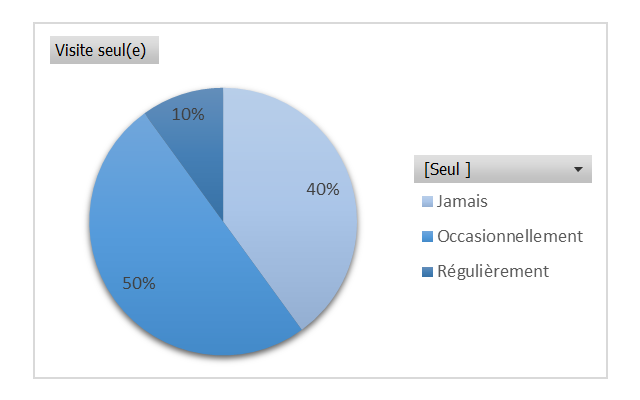
\includegraphics[width=\textwidth]{figures/visiteseul.png}
\end{minipage} \hfill
\begin{minipage}{.49\textwidth}
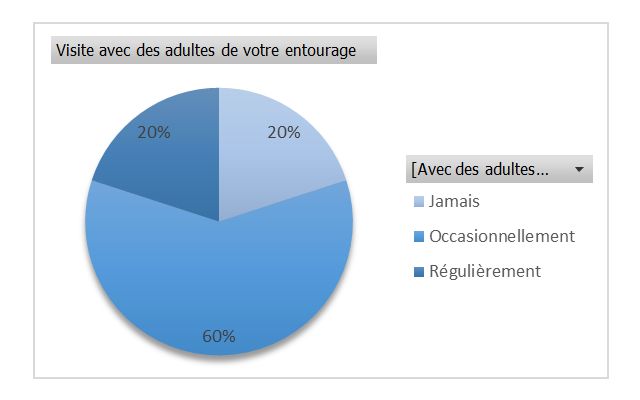
\includegraphics[width=\textwidth]{figures/visiteadulte.png}
\end{minipage}

\begin{minipage}{.49\textwidth}
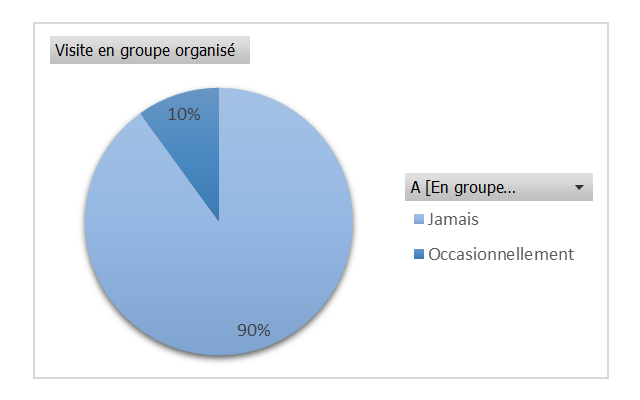
\includegraphics[width=\textwidth]{figures/visitegroupe.png}
\end{minipage} \hfill
\begin{minipage}{.49\textwidth}
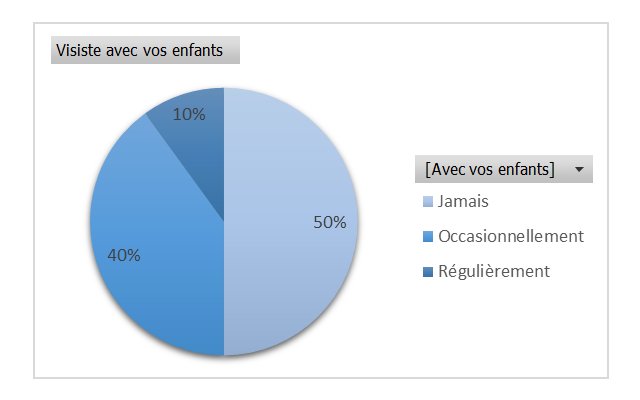
\includegraphics[width=\textwidth]{figures/visiteenfant.png}
\end{minipage}

\caption{Répartition des groupes de personnes en fonction de leur habitude de visite.}%
\label{fig:groupePersonnes}%
\end{figure}


\section{Séances participatives}

\subsection{Séance 1}

La première séance avait pour but d'obtenir une vue générale des possibilités d'applications du dispositif GUIMUTEIC.
Elle devait répondre aux objectifs suivants : 
\begin{itemize}
	\item Connaître les pratiques actuelles des participants lors de visite de musée/monument;
	\item Avoir la perception et le ressenti vis-à-vis du dispositif prévu;
	\item Définir des modes d'interaction souhaités;
	\item Définir des fonctionnalités innovantes souhaitées.
\end{itemize}

Suite à cette séance, les fonctionnalitées préférées par les participants sont : 
\begin{itemize}
\item L’analyse du regard pour proposer des informations correspondantes
\item L’orientation du visiteur en fonction d’un parcours de visite
\item La commande vocale
\item Le contrôle à base de gestes
\end{itemize}

Les participants ont relevé deux utilisations distincts du dispositif GUIMUTEIC : un assistant de visite et un guide de visite.
Un assistant intervient lors de la visite pour apporter des informations complémentaires sous forme de commentaire audio ou vidéo.
Un guide oriente l’utilisateur en fonction d’un parcours prédéfini ou personnalisé pour le visiteur en fonction de son temps, ses connaissance, etc.

Un point important soulevé est que les participants privilégient l’utilisation de l’appareil de manière autonome. Ils ne souhaitent pas un objet supplémentaire pour l’utiliser.

Un certain nombre de souhaits sur le dispositifs ont été émis: 
\begin{itemize}
\item Avoir un seul écouteur ou un casque ouvert pour pallier au sentiment d’isolement;
\item Pouvoir orienter la caméra vers l’oeuvre;
\item Pour relever l’écran quand l’utilisateur ne souhaite pas l’utiliser.
\end{itemize}





 \subsection{Séance 2}

L’objectif de la deuxième séance était de déterminer l’intérêt d’un écran sur le dispositif, ainsi que l’ergonomie du casque, avec les buts suivants: 
\begin{itemize}
	\item Connaître le ressenti des participants vis-à-vis du dispositif.
	\item Définir l'interaction lors du parcours de visite.
	\item Identifier les gestes pertinents.
\end{itemize}

La présence d’un écran est jugé inutile si l’écran est trop petit. 
Le casque présenté avait un écran du même type de les GoogleGlass\footnote{\url{www.google.com}}, mais rabattable.
Les participants l’ont jugé trop petit pour être utilisable pendant une longue visite.
De plus, la branche utilisée pour rabattre l’écran est perçue comme trop imposante et non adaptée aux enfants.

Un certain nombre de gestes sont proposés par les participants pour réaliser l'interaction.
Les gestes suivants, qui n’ont pas été retenus car ils requièrent un certain niveau d’apprentissage : sauvegarder et reprendre.
Deux autres gestes n’ont pas été retenus car ils sont similaires (voir figure~\ref{fig:gestes1}): sélectionner et démarrer.


\begin{figure}%
\centering
\begin{subfigure}{0.48\textwidth}
\includegraphics[width=\columnwidth]{figures/gestes/démarrer.png}%
\caption{Démarrer}
\end{subfigure}
\begin{subfigure}{0.48\textwidth}
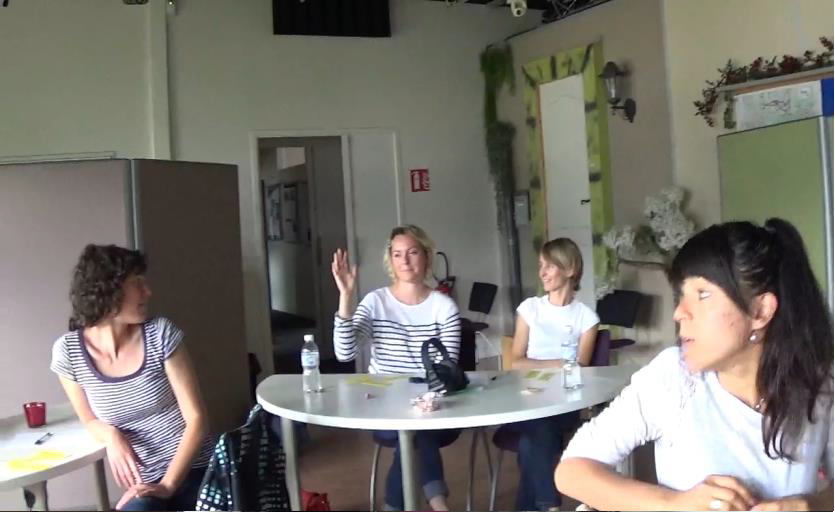
\includegraphics[width=\columnwidth]{figures/gestes/selectionner.png}%
\caption{Sélectionner}
\end{subfigure}

\caption{Gestes Sélectionner et Démarrer identifiés lors des séances participatives}%
\label{fig:gestes1}%
\end{figure}

Il ressort de cette séance que les participants sont enclins à utiliser des gestes, si ceux-ci sont ``intuitifs et universels''.
Ils ne souhaitent pas apprendre de nouveaux gestes. 
Certains avancent le fait qu’utiliser des gestes peut permettre de rendre l'interaction plus fluide et rapide.
En revanche, ils insistent sur la rapidité et la qualité de la reconnaissance, qui doit être immédiate sous peine d’être rejetée par les utilisateurs.
Le geste le plus demandé est le pointage, pour déclencher le guide sur une oeuvre donnée.


\subsection{Séance 3}

La troisième séance devait répondre aux objectifs suivants :
\begin{itemize}
\item Définir l’ergonomie du casque (écouteur, écran, …);
\item Identifier les gestes et les modes d’interactions pertinents
\end{itemize}

Durant cette séance, les participants ont été invités à dessiner l'appareil idéal pour chacun.
Les dessins sont ensuite soumis aux votes.
Sur la figure~\ref{fig:dessins}, on voit les dessins qui ont reçu le plus de votes.
Le premier propose un écran et des écouteurs amovibles, avec une zone tactile au niveau des écouteurs pour le contrôle de l’appareil.
La deuxième proposition est un système à base de lunettes, avec des écouteurs amovibles. L’interaction se fait alors par la reconnaissances des mouvements oculaires ou avec une télécommande.
Le troisième dessin propose un écran semi-opaque et des écouteurs amovibles. L’interaction se fait également avec reconnaissance de mouvements oculaires.

\begin{figure}%
\centering
\begin{subfigure}{0.32\textwidth}
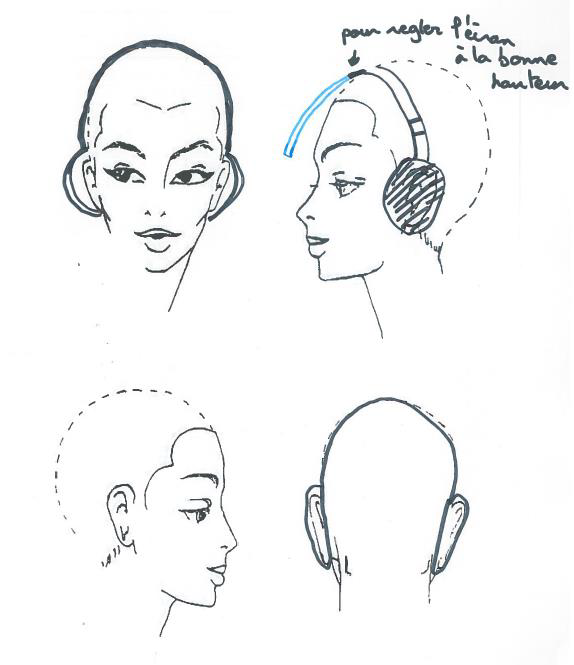
\includegraphics[width=\columnwidth]{figures/gestes/dessincasque.png}%
\caption{Dessin 1}
\end{subfigure}
\begin{subfigure}{0.32\textwidth}
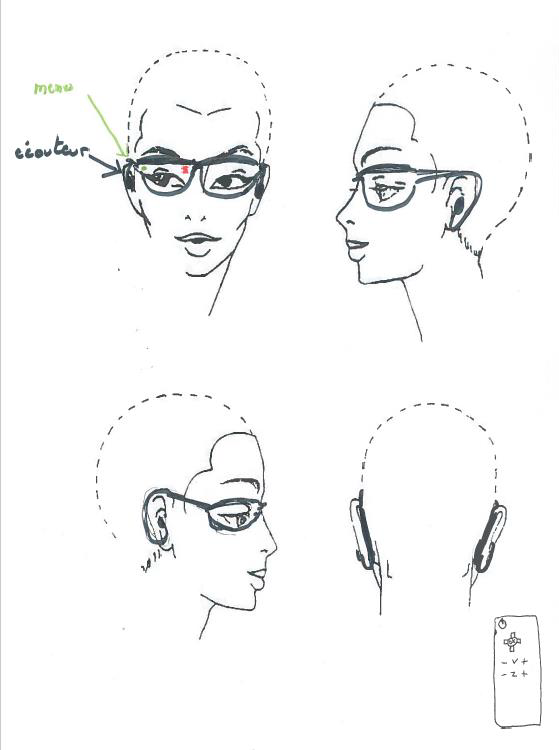
\includegraphics[width=\columnwidth]{figures/gestes/dessincasque2.png}%
\caption{Dessin 2}
\end{subfigure}
\begin{subfigure}{0.32\textwidth}
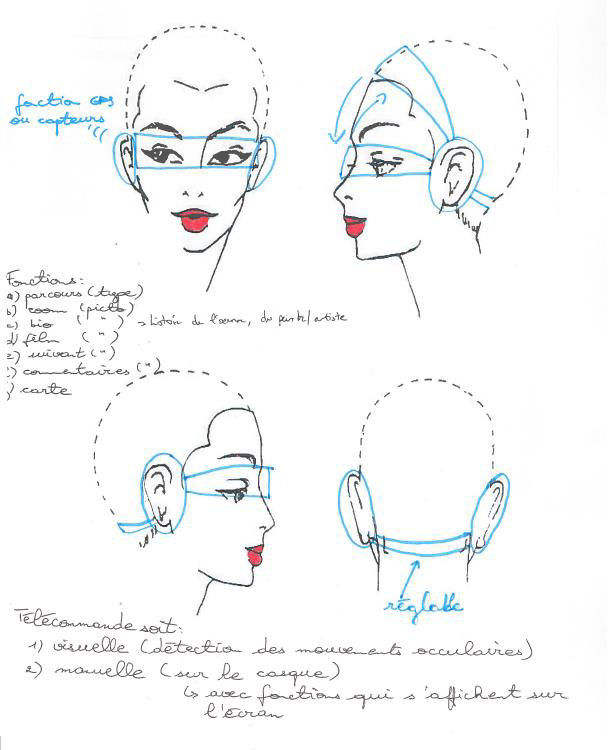
\includegraphics[width=\columnwidth]{figures/gestes/dessincasque3.png}%
\caption{Dessin 2}
\end{subfigure}


\caption{Gestes Sélectionner et Démarrer identifiés lors des séances participatives}%
\label{fig:dessins}%
\end{figure}


Le bilan de cette séance est que le casque doit être réglable, et surtout amovible, pour ne pas couper l’utilisateur de reste du monde. Les écouteurs doivent être amovibles ou ouverts, et l’interaction doit être fait sans appareil supplémentaire.


\section{Bilan}

D nombreux éléments pour le dispositif GUIMUTEIC peuvent être retenus de ces séances de conceptions participatives.
Tout d’abord au niveau du guide, un choix entre une aide forte, avec guidage du visiteur, et une aide simple, qui n’intervient que lorsque qu’on lui demande, est important.
Ensuite, au niveau du dispositif, la flexibilité de son utilisation est un point soulevé par de nombreux participants.
Les écouteurs doivent être amovibles ou ouverts, pour que le visiteur puisse communiquer avec d’autres personnes s’il le désire.
Si un écran est disponible, il doit être rabattable, pour ne pas gêner l’utilisateur.

Au niveau de l’interaction avec l’appareil, un consensus sur le fait qu’il ne faut pas manipuler l'appareil supplémentaire est apparu.
L’analyse de mouvement oculaire est revenue plusieurs fois, mais n’est pas compatible avec un écran rabattable, en plus d’être difficile à mettre en place pour un appareil destiné au grand public. 
L’interaction à base de commande vocale est bien accueilli, mais difficilement utilisable dans un musée.
Les gestes sont donc ce qu’il faut retenir dans ce cas pour une interaction adaptée, si la reconnaissance est assez rapide et précise. 


%%%%%%%%%%%%%%%%%%%%%%%%%%%%%%%%%%%%%%%%%%%%%%%%%%%%%
%
%
%			Code et schémas
%
%
%%%%%%%%%%%%%%%%%%%%%%%%%%%%%%%%%%%%%%%%%%%%%%%%%%%%%%
\chapter{Réseau de reconnaissance de gestes}


Cette section présente le code et les schémas des blocs et du réseau présentés dans la chapitre~\ref{chap:gestes}. 
Le code est en python, pour le framework PyTorch, et permet de voir les détails de l'implémentation de chacun des blocs.
Les schémas sont des compléments à la figure~\ref{fig:reseau1}, qui ne présentait qu'un des exemples d'architecture utilisé pour la courbe~\ref{fig:FusionLayer}.
Nous fournissons également les schémas des architecture ShuffleNet et ResNet modifier pour réaliser la fusion des informations, présentés dans le tableau~\ref{tab:fusion}.


\section{Implémentation}
\label{sec:implementation}

\subsection{Bloc S1-FrameWise}
\label{sec:implementationS1}

\begin{lstlisting}[language=Python]
class S1FW(nn.Module):
    """
        S1 FrameWise module
        inputs : 
           * inp = number of input channel
           * outp = number of output channel
           * nbf = number of frames
    """
    
    def __init__(self,inp, outp, nbf=1):
        super(S1FW, self).__init__()
        #	deepwise 3*3 convolution 
        self.conv3 = nn.Conv2d(inp*nbf, inp*nbf, 
                              kernel_size=3, stride=1,
                              padding=1, groups=inp*nbf)
        self.bn3 = nn.BatchNorm2d(inp*nbf)
				# framewise 1*1 convolution
        self.conv1 = nn.Conv2d(inp*nbf, outp*nbf, 
                              kernel_size=1, stride=1, 
                              padding=0, groups=nbf)
        self.bn1 = nn.BatchNorm2d(outp*nbf)
        self.relu = nn.ReLU(True)
        
    def forward(self, x):
        right = self.relu(self.bn3(self.conv3(x)))
        right = self.relu(self.bn1(self.conv1(right)))
        return x.add(right)
\end{lstlisting}


\subsection{Bloc S2-FrameWise}
\label{sec:implementationS2}

\begin{lstlisting}[language=Python]
class S2FW(nn.Module):
    """
        S2 FrameWise module
        inputs : 
           * inp = number of input channel
           * outp = number of output channel
           * nbf = number of frames
    """
    def __init__(self,inp, outp, nbf=1):
        super(S2FW, self).__init__()
        #	deepwise 3*3 convolution 
        self.conv3     = nn.Conv2d(inp*nbf, inp*nbf, 
                                   kernel_size=3, stride=2, padding=1, groups=inp*nbf)
        self.bn3       = nn.BatchNorm2d(inp*nbf)
        # framewise 1*1 convolution
        self.conv1     = nn.Conv2d(inp*nbf, outp*nbf, kernel_size=1, stride=1, padding=0, groups=nbf)
        self.bn1       = nn.BatchNorm2d(outp*nbf)
        self.relu      = nn.ReLU()
        self.pool      = nn.AvgPool2d(kernel_size=3, padding=1, stride=2)
        
    def forward(self, x):
        left = self.pool(x)
        right = self.relu(self.bn3(self.conv3(x)))
        if self.shuffle:
            right = channel_shuffle(right, self.nb_groups)
        right = self.relu(self.bn1(self.conv1(right)))
        return torch.cat( (left, right), 1)
\end{lstlisting}


\subsection{Réseau multi-trame}
\label{sec:implementationRMF}


\begin{lstlisting}[language=Python]
class DenseMobile(nn.Module):
    def __init__(self, in_channel=3, nb_frames=3, num_classes=6):
        super(DenseMobile, self).__init__()

        self.blocStart = DownBloc(in_channel, 32-in_channel, in_channel, nb_frames=nb_frames) #224x224x3 -> 112x112x32
        self.features = nn.Sequential(
                        S1FW(32,32,nb_frames), # -> 112x112x32xnb_frame
                        S2FW(32,32,nb_frames), # -> 56x56x64xnb_frame
                        S1FW(64,64,nb_frames), # -> 56x56x128xnb_frame
                        S2FW(64, 192,nb_frames), # -> 28x28x256xnb_frame
                        FusionBloc(256,256, nb_frames),-> 28x28x256
                        S1(256,256, 256), # -> 28x28x256
                        S2(256, 256, 256), # -> 14x14x512
                        S1(512, 512, 512), # -> 28x28x256
												S2(512,512,512), # -> 7x7x1024
												nn.AvgPool2d(kernel_size=7, padding=0, stride=1), #3x3
                    )
        
        self.classif = nn.Linear(1024, num_classes)
        
    def forward(self, x):
        x = self.blocStart(x)
        x = self.features(x)
        return self.classif(x.view(x.size(0),-1))
\end{lstlisting}


\section{Fusion des informations}

\subsection{Réseau multi-frame}
\label{sec:multiframeSchemas}


\begin{figure}%
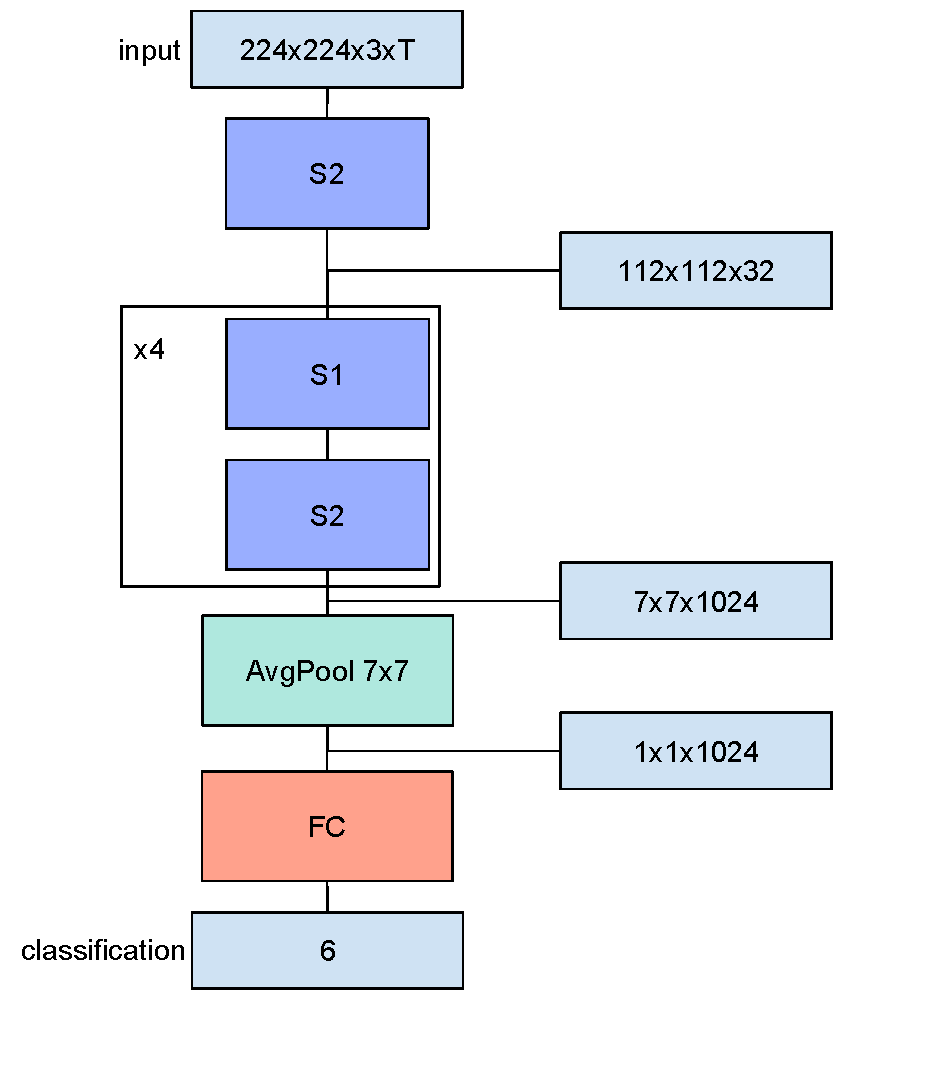
\includegraphics[width=\columnwidth]{figures/Reseau1Fusion1.pdf}%
\caption{Fusion 1}%
\label{fig:fusion1}%
\end{figure}


\begin{figure}%
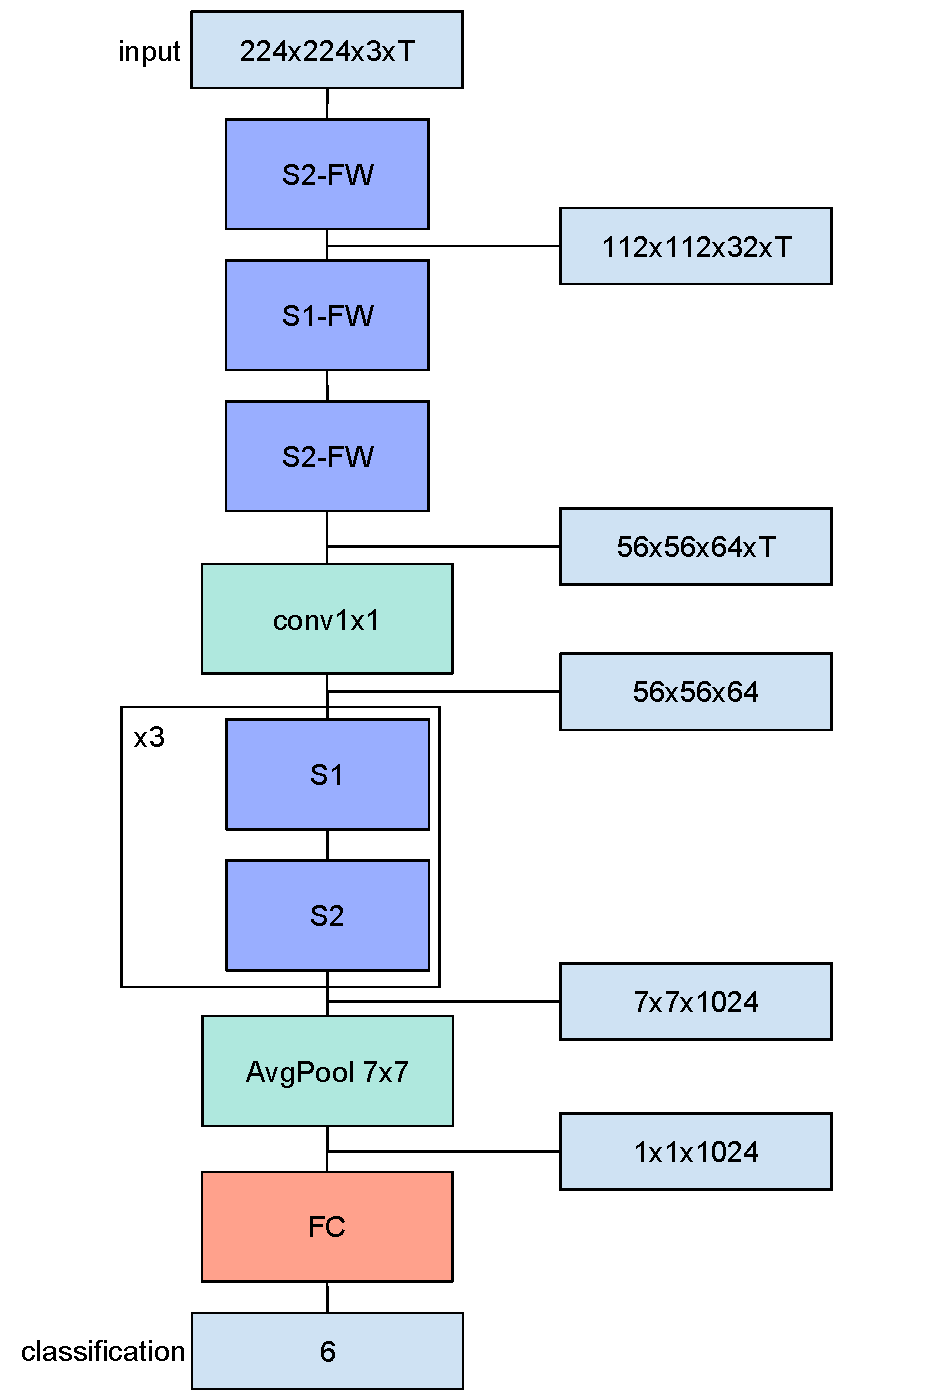
\includegraphics[width=\columnwidth]{figures/Reseau1Fusion2.pdf}%
\caption{Fusion 2}%
\label{fig:fusion2}%
\end{figure}


\begin{figure}%
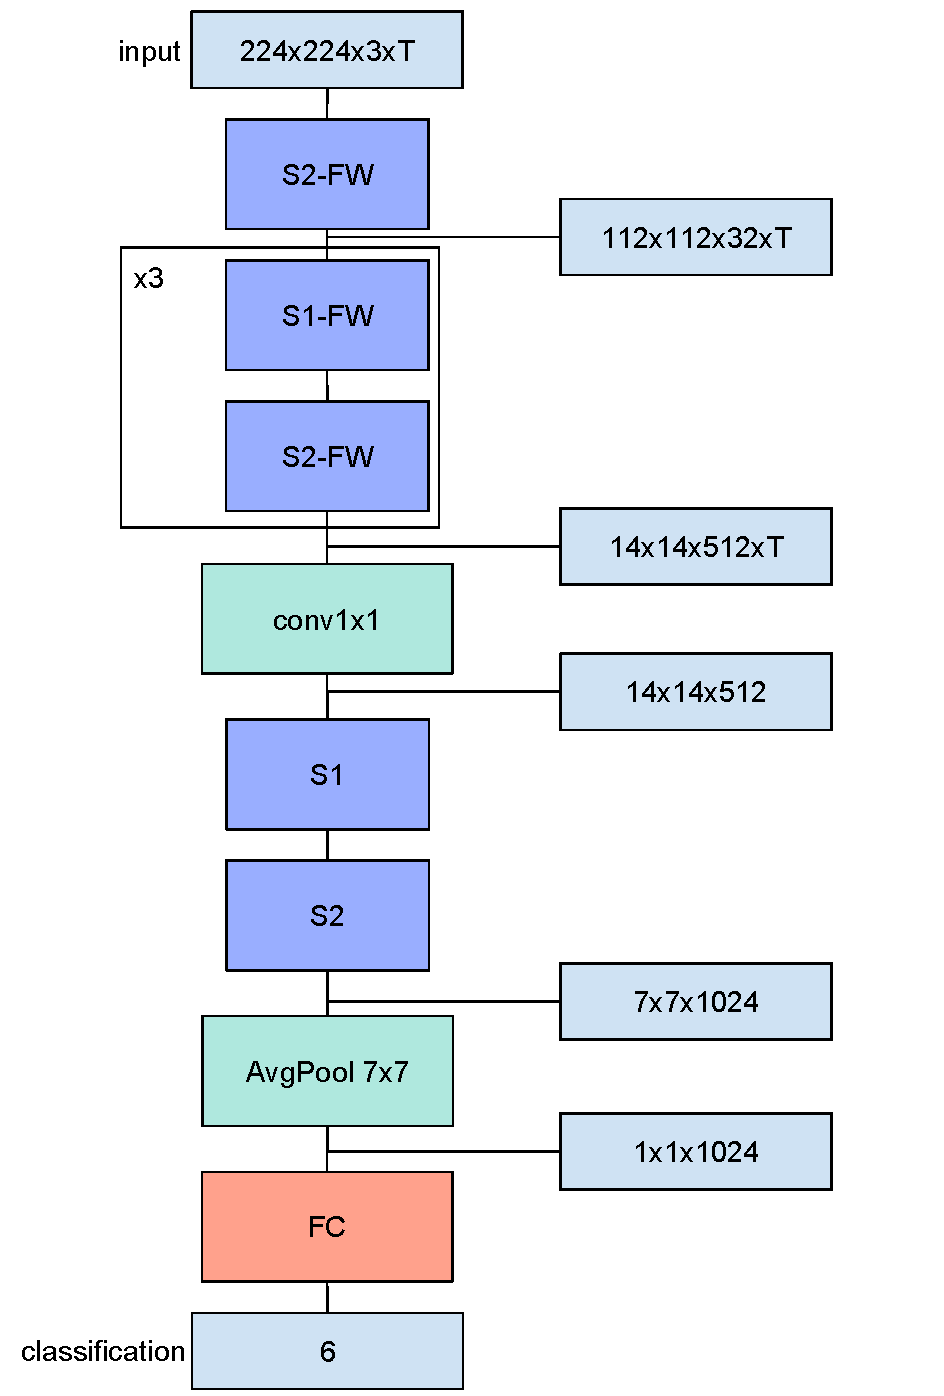
\includegraphics[width=\columnwidth]{figures/Reseau1Fusion4.pdf}%
\caption{Fusion 4}%
\label{fig:fusion4}%
\end{figure}


\begin{figure}%
\includegraphics[width=\columnwidth]{figures/Reseau1Fusion5.pdf}%
\caption{Fusion 5}%
\label{fig:fusion5}%
\end{figure}


%\subsection{ShuffleNet multi-trames}
%
%
%\begin{figure}%
%%\includegraphics[width=\columnwidth]{filename}%
%\caption{ShuffleNet avec fusion sur la première couche}%
%\label{fig:shuffleF1}%
%\end{figure}
%
%
%\begin{figure}%
%%\includegraphics[width=\columnwidth]{filename}%
%\caption{ShuffleNet avec fusion au milieu de réseau}%
%\label{fig:shuffleFM}%
%\end{figure}
%
%
%
%\begin{figure}%
%%\includegraphics[width=\columnwidth]{filename}%
%\caption{ShuffleNet avec fusion sur la dernière couche}%
%\label{fig:shuffleFFC}%
%\end{figure}
%
%
%
%\subsection{ResNet multi-trames}
%
%
%\begin{figure}%
%%\includegraphics[width=\columnwidth]{filename}%
%\caption{ResNet avec fusion sur la première couche}%
%\label{fig:resnetF1}%
%\end{figure}
%
%
%\begin{figure}%
%%\includegraphics[width=\columnwidth]{filename}%
%\caption{ResNet avec fusion sur la dernière couche}%
%\label{fig:resnetFFC}%
%\end{figure}
%
%
%
%\begin{figure}%
%%\includegraphics[width=\columnwidth]{filename}%
%\caption{ResNet avec fusion grâce à une couche LSTM}%
%\label{fig:resnetFLSTM}%
%\end{figure}



